% Options for packages loaded elsewhere
\PassOptionsToPackage{unicode}{hyperref}
\PassOptionsToPackage{hyphens}{url}
%
\documentclass[
]{article}
\usepackage{lmodern}
\usepackage{amssymb,amsmath}
\usepackage{ifxetex,ifluatex}
\ifnum 0\ifxetex 1\fi\ifluatex 1\fi=0 % if pdftex
  \usepackage[T1]{fontenc}
  \usepackage[utf8]{inputenc}
  \usepackage{textcomp} % provide euro and other symbols
\else % if luatex or xetex
  \usepackage{unicode-math}
  \defaultfontfeatures{Scale=MatchLowercase}
  \defaultfontfeatures[\rmfamily]{Ligatures=TeX,Scale=1}
\fi
% Use upquote if available, for straight quotes in verbatim environments
\IfFileExists{upquote.sty}{\usepackage{upquote}}{}
\IfFileExists{microtype.sty}{% use microtype if available
  \usepackage[]{microtype}
  \UseMicrotypeSet[protrusion]{basicmath} % disable protrusion for tt fonts
}{}
\makeatletter
\@ifundefined{KOMAClassName}{% if non-KOMA class
  \IfFileExists{parskip.sty}{%
    \usepackage{parskip}
  }{% else
    \setlength{\parindent}{0pt}
    \setlength{\parskip}{6pt plus 2pt minus 1pt}}
}{% if KOMA class
  \KOMAoptions{parskip=half}}
\makeatother
\usepackage{xcolor}
\IfFileExists{xurl.sty}{\usepackage{xurl}}{} % add URL line breaks if available
\IfFileExists{bookmark.sty}{\usepackage{bookmark}}{\usepackage{hyperref}}
\hypersetup{
  pdftitle={Case Study of BellaBeat Health Tracker},
  hidelinks,
  pdfcreator={LaTeX via pandoc}}
\urlstyle{same} % disable monospaced font for URLs
\usepackage[margin=1in]{geometry}
\usepackage{graphicx}
\makeatletter
\def\maxwidth{\ifdim\Gin@nat@width>\linewidth\linewidth\else\Gin@nat@width\fi}
\def\maxheight{\ifdim\Gin@nat@height>\textheight\textheight\else\Gin@nat@height\fi}
\makeatother
% Scale images if necessary, so that they will not overflow the page
% margins by default, and it is still possible to overwrite the defaults
% using explicit options in \includegraphics[width, height, ...]{}
\setkeys{Gin}{width=\maxwidth,height=\maxheight,keepaspectratio}
% Set default figure placement to htbp
\makeatletter
\def\fps@figure{htbp}
\makeatother
\setlength{\emergencystretch}{3em} % prevent overfull lines
\providecommand{\tightlist}{%
  \setlength{\itemsep}{0pt}\setlength{\parskip}{0pt}}
\setcounter{secnumdepth}{-\maxdimen} % remove section numbering
\usepackage{booktabs}
\usepackage{longtable}
\usepackage{array}
\usepackage{multirow}
\usepackage{wrapfig}
\usepackage{float}
\usepackage{colortbl}
\usepackage{pdflscape}
\usepackage{tabu}
\usepackage{threeparttable}
\usepackage{threeparttablex}
\usepackage[normalem]{ulem}
\usepackage{makecell}
\usepackage{xcolor}

\title{Case Study of BellaBeat Health Tracker}
\usepackage{etoolbox}
\makeatletter
\providecommand{\subtitle}[1]{% add subtitle to \maketitle
  \apptocmd{\@title}{\par {\large #1 \par}}{}{}
}
\makeatother
\subtitle{Improving Marketing Strategy With}
\author{}
\date{\vspace{-2.5em}}

\begin{document}
\maketitle

\hypertarget{summary}{%
\section{Summary}\label{summary}}

In this case study I am going to analyze data from FitBit users, which
is a personal health tracker. The objective is to gain insights from
FitBit secondary data, to drive business decisions for another health
tracker company called BellaBeat. This data analysis can help guide
BellaBeat's marketing strategies, particularly for two of their products
Leaf (tracker bracelet) and Time (wellness watch). Their main feature is
tracking and measuring user wellness activities by connecting to
BellaBeat app. Then the app provides users with insights into their
daily wellness, using attributes such as sleep, weight, calories burnt,
menstrual cycle, and mindfulness habits. I am going to analize FitBit
data to find the most important problems BellaBeat might face and come
up with recommendations on what tools to implement to solve them. The
datasets and some instructions were provided by Google Data Analytics,
which is a course on Cursera, developed by Google. The datasets are not
perfect and have some limitations. The purpose is not to pass over these
limitations, and make it seem like the analysis is perfectly accurate,
but rather to face the limitations and discuss some possible ways to
avoid them in the future. These limitations commonly occur in many
similar datasets in practice. Hence, it may be useful to discuss them
thoroughly.

So, the business task is, essentially, to provide BellaBeat with
recommendations for their marketing strategy. To reach that goal, the
main approach used in the case study is to follow these steps: first to
develop a scenario, then understand what the stakeholders would be
interested in (deliverable), pre-determine some guiding questions. Then
proceed with data analysis process to find answers that lead to the
desired recommendations for the marketing team. Here the analysis
processes involves the following phases: Data Preparation, Data Cleaning
and Processing, Analyze and Visualize. This case study is divided into
sections and subsections (refer to the table of content). Following this
summary each section can be viewed as one of the data analysis phases
(in the same order), which commonly seen in the real world. These phases
are sometimes refereed to as ask questions, prepare data, process/clean
data, share and act.

\hypertarget{deliverables}{%
\paragraph{Deliverables}\label{deliverables}}

\begin{enumerate}
\def\labelenumi{\arabic{enumi}.}
\tightlist
\item
  A clear summary of the business task
\item
  A description of all data sources used
\item
  Documentation of any cleaning or manipulation of data
\item
  A summary of your analysis
\item
  Supporting visualizations and key findings
\item
  Your top high-level content recommendations based on your analysis
\end{enumerate}

\hypertarget{questions-to-address}{%
\paragraph{Questions to address}\label{questions-to-address}}

\begin{enumerate}
\def\labelenumi{\arabic{enumi}.}
\tightlist
\item
  What are some trends in smart device usage?
\item
  How could these trends apply to BellaBeat customers?
\item
  How could these trends help influence BellaBeat marketing strategy?
\end{enumerate}

\hypertarget{data-preparation}{%
\section{Data Preparation}\label{data-preparation}}

In this step, we need to prepare data for processing and analyzing. We
will need to take a close look at the datasets, summarize them and
discover some data quality characteristics. To do so, we need to examine
each dataset closely. Originally there where 18 available FitBit
datasets that were obtained from Kaggle(XXXX add link). Of the 18
original datasets only 12 were used, since some columns repeated across
the datasets and some of them did not fit into the context of this case
study problems.

\hypertarget{data-summary}{%
\paragraph{Data Summary:}\label{data-summary}}

Bellow I created metadata of the datasets that encompasses some of the
important data quality characteristics:

\begin{table}
\centering
\begin{tabular}[t]{>{}l||>{\raggedright\arraybackslash}p{30em}|l|r|r|r}
\hline
Datasets & Variables & Num.of.Unique.Ids & Num.of.Variables & Num.of.Rows & Missing.Values\\
\hline
\textbf{dailyActivity_merged . csv} & Id, ActivityDate, TotalSteps, TotalDistance, TrackerDistance, LoggedActivitiesDistance, VeryActiveDistance, ModeratelyActiveDistance, LightActiveDistance, SedentaryActiveDistance, VeryActiveMinutes, FairlyActiveMinutes, LightlyActiveMinutes, SedentaryMinutes, Calories & \textcolor{black}{33} & 15 & 940 & 0\\
\hline
\textbf{heartrate_seconds_merged . csv} & Id, Time, Value & \textcolor{red}{14} & 3 & 2483658 & 0\\
\hline
\textbf{hourlyCalories_merged . csv} & Id, ActivityHour, Calories & \textcolor{black}{33} & 3 & 22099 & 0\\
\hline
\textbf{hourlyIntensities_merged . csv} & Id, ActivityHour, TotalIntensity, AverageIntensity & \textcolor{black}{33} & 4 & 22099 & 0\\
\hline
\textbf{hourlySteps_merged . csv} & Id, ActivityHour, StepTotal & \textcolor{black}{33} & 3 & 22099 & 0\\
\hline
\textbf{minuteCaloriesNarrow_merged . csv} & Id, ActivityMinute, Calories & \textcolor{black}{33} & 3 & 1325580 & 0\\
\hline
\textbf{minuteIntensitiesNarrow_merged . csv} & Id, ActivityMinute, Intensity & \textcolor{black}{33} & 3 & 1325580 & 0\\
\hline
\textbf{minuteMETsNarrow_merged . csv} & Id, ActivityMinute, METs & \textcolor{black}{33} & 3 & 1325580 & 0\\
\hline
\textbf{minuteSleep_merged . csv} & Id, date, value, logId & \textcolor{red}{24} & 4 & 188521 & 0\\
\hline
\textbf{minuteStepsNarrow_merged . csv} & Id, ActivityMinute, Steps & \textcolor{black}{33} & 3 & 1325580 & 0\\
\hline
\textbf{sleepDay_merged . csv} & Id, SleepDay, TotalSleepRecords, TotalMinutesAsleep, TotalTimeInBed & \textcolor{red}{24} & 5 & 413 & 0\\
\hline
\textbf{weightLogInfo_merged . csv} & Id, Date, WeightKg, WeightPounds, Fat, BMI, IsManualReport, LogId & \textcolor{red}{8} & 8 & 67 & 65\\
\hline
\end{tabular}
\end{table}

\hypertarget{data-limitations}{%
\paragraph{Data Limitations:}\label{data-limitations}}

There are some limitations found. First and foremost, the datasets have
inputs of only 33 unique users. This tells us that the data is not
comprehensive. Of the 33 users only 8 entered weight, 12 heart rate and
only 24 users for sleep entries. Moreover, within the weight dataset
some users did not enter information for all the variables. This means
that the data is also incomplete and hence \textbf{not comprehensive}.
However, since all of these 3 datasets are comprised of important
variables, we will still work with those.

The data comes from FitBit users, which is a second source. This tells
us the data is \textbf{not original}. It means that the data may lead to
inaccurate insights, since the user behavior and the data distribution
of FitBit is not the same as that of BellaBeat.

Another limitation is that the data is \textbf{not current}. The dates
at which the data was collected ranges from 4/12/2016 to 5/12/2016,
which was about 5 years before the time of this case study.

Another limitation that will most likely affect data integrity is that
the data was only collected for only 30 days. So, having only 33 users'
data, 30 entries each, will effect the reliability. Moreover we are
expecting 30x33=990 rows, however, there are 940 in the daily dataset.
This means that some users either did not enter the information, were
not wearing the tracker or the device did not collect the data properly.
Also some of values were entered manually, for instance, that of the
weight information. These and some other complications might resulted in
a \textbf{biased} data.

Had this been a real-life project that would intend to define
BellaBeat's marketing strategy, these limitations would have been
addressed before stating the analysis phrase. However, Since this is a
case study, and we do not have control over these limitations, we will
still proceed to the analysis. Though, we should mention the type of
questions that the data analyst would ask in a real world scenario,
before proceeding with the data cleaning. Here they are:

\begin{itemize}
\tightlist
\item
  Why some users generated more data rows then others. Is it a device
  data collection system or did they turn them off ?
\item
  Did users volunteerly contributed data or at their convenience or were
  they told how often and when to use the app ?
\item
  Is it possible to know what what measures were taken to eliminate the
  sampling bias ?
\item
  Is it possible to obtain the newer version of these dataets dataset ?
\item
  Is it possible to obtain similar dataset from BellaBeat for
  originality ?
\end{itemize}

\hypertarget{data-privacy}{%
\paragraph{Data Privacy}\label{data-privacy}}

BealaBeat's website provides a thorough data privacy section. Also
comparing with its competitors, it seems to be well developed. Just
looking at the first glance it is seems that BellaBeat can collect
valuable data from its users and develop marketing strategies based on
the data users provide, without revealing their identity or selling to
another company. It needs further research to determine the validity of
these assumptions. I will leave it to the reader and in the References
section provide links that might help.

\hypertarget{data-cleaning-and-processing}{%
\section{Data Cleaning And
Processing}\label{data-cleaning-and-processing}}

So, we already prepared ground for data processing in the data prep
section. Since we decided that we should proceed with the analysis,
despite the limitations, we will start the cleaning process. Our focus
here should be on discussing data integrity and some risk that may rise
if it's violated. One should note that most likely some integrity issues
can not be resolved in these case study. This is because we we won't be
able to communicate with the stakeholders and request what we need. For
instance we found that there were only 8 users who had inputs for weight
information. This is a huge problem, since it may lead to wrong
conclusions. However, we will determine those issues and ignore them for
learning purposes. But keep in mind that in a real-life situation, for a
strong analysis, a data analyst would have to do what it takes to ensure
data integrity, and only then proceed with the analysis phrase.

Before we do the cleaning, we will take a first look at some of the key
datasets and their attributes for illustration purposes. The tables
bellow represent the first few observations of the first two users in
the dataset. Note that the tables are scrollable, so feel free to
explore more rows and columns.

\textbackslash begin\{table\}

\caption{\label{tab:unnamed-chunk-4}Scrollable tables}

\textbackslash begin\{table\}

\textbackslash caption\{\label{tab:unnamed-chunk-4} \textbf{Table 1.}
minuteCaloriesNarrow\_merged.csv\} \centering

\begin{tabular}[t]{r|r|r}
\hline
Id & ActivityMinute & Calories\\
\hline
1503960366 & 4/12/2016 12:00:00 AM & 0.7865\\
\hline
1503960366 & 4/12/2016 12:01:00 AM & 0.7865\\
\hline
1503960366 & 4/12/2016 12:02:00 AM & 0.7865\\
\hline
1503960366 & 4/12/2016 12:03:00 AM & 0.7865\\
\hline
1503960366 & 4/12/2016 12:04:00 AM & 0.7865\\
\hline
1624580081 & 4/12/2016 12:00:00 AM & 0.8310\\
\hline
1624580081 & 4/12/2016 12:01:00 AM & 0.8310\\
\hline
1624580081 & 4/12/2016 12:02:00 AM & 0.8310\\
\hline
1624580081 & 4/12/2016 12:03:00 AM & 0.8310\\
\hline
1624580081 & 4/12/2016 12:04:00 AM & 0.8310\\
\hline
\end{tabular}

\textbackslash end\{table\}\textbackslash begin\{table\}

\textbackslash caption\{\label{tab:unnamed-chunk-4} \textbf{Table 2.}
minuteSleep\_merged.csv\} \centering

\begin{tabular}[t]{r|r|r|r}
\hline
Id & date & value & logId\\
\hline
1503960366 & 4/12/2016 2:47:30 AM & 3 & 11380564589\\
\hline
1503960366 & 4/12/2016 2:48:30 AM & 2 & 11380564589\\
\hline
1503960366 & 4/12/2016 2:49:30 AM & 1 & 11380564589\\
\hline
1503960366 & 4/12/2016 2:50:30 AM & 1 & 11380564589\\
\hline
1503960366 & 4/12/2016 2:51:30 AM & 1 & 11380564589\\
\hline
1644430081 & 4/29/2016 6:33:30 PM & 1 & 11523617009\\
\hline
1644430081 & 4/29/2016 6:34:30 PM & 1 & 11523617009\\
\hline
1644430081 & 4/29/2016 6:35:30 PM & 1 & 11523617009\\
\hline
1644430081 & 4/29/2016 6:36:30 PM & 1 & 11523617009\\
\hline
1644430081 & 4/29/2016 6:37:30 PM & 1 & 11523617009\\
\hline
\end{tabular}

\textbackslash end\{table\} \textbackslash end\{table\}

\textbackslash begin\{table\} \textbackslash begin\{table\}

\textbackslash caption\{\label{tab:unnamed-chunk-4} \textbf{Table 3.}
heartrate\_seconds\_merged.csv\} \centering

\begin{tabular}[t]{r|r|r}
\hline
Id & Time & Value\\
\hline
2022484408 & 4/12/2016 7:21:00 AM & 97\\
\hline
2022484408 & 4/12/2016 7:21:05 AM & 102\\
\hline
2022484408 & 4/12/2016 7:21:10 AM & 105\\
\hline
2022484408 & 4/12/2016 7:21:20 AM & 103\\
\hline
2022484408 & 4/12/2016 7:21:25 AM & 101\\
\hline
2026352035 & 4/17/2016 5:30:20 AM & 70\\
\hline
2026352035 & 4/17/2016 5:30:30 AM & 66\\
\hline
2026352035 & 4/17/2016 5:30:40 AM & 67\\
\hline
2026352035 & 4/17/2016 5:30:55 AM & 67\\
\hline
2026352035 & 4/17/2016 5:31:10 AM & 67\\
\hline
\end{tabular}

\textbackslash end\{table\}\textbackslash begin\{table\}

\textbackslash caption\{\label{tab:unnamed-chunk-4} \textbf{Table 4.}
weightLogInfo\_merged.csv\} \centering

\begin{tabular}[t]{r|r|r|r|r|r|r|r}
\hline
Id & Date & WeightKg & WeightPounds & Fat & BMI & IsManualReport & LogId\\
\hline
1503960366 & 5/2/2016 11:59:59 PM & 52.6 & 115.9631 & 22 & 22.65 & True & 1.462234e+12\\
\hline
1503960366 & 5/3/2016 11:59:59 PM & 52.6 & 115.9631 & NA & 22.65 & True & 1.462320e+12\\
\hline
1927972279 & 4/13/2016 1:08:52 AM & 133.5 & 294.3171 & NA & 47.54 & False & 1.460510e+12\\
\hline
\end{tabular}

\textbackslash end\{table\} \textbackslash end\{table\} /

In the upcoming paragraphs I will provide a high level description of
the steps I took to ensure that the data is clean. Of course, the data
cleaning procedure involved a lot of effort and I may not describe some
of them here. But it can be found in the scripts and by looking at the
comments. So, the data cleaning strategy I used for this case study
involves but is not limited to the following steps:

\hypertarget{alignment-with-objectives-merge}{%
\paragraph{Alignment with objectives
(merge)}\label{alignment-with-objectives-merge}}

Essential, the purpose of this step is to bring the data into a desired
format and align with case study objectives. This includes making
necessary transformations and removing the irrelevant information and
organizing the datasets in a way that is suitable and makes it easy to
analyze.

\textbf{Transformation.} Looking at the 4 datasets above we see that
they all have a column \textbf{Id}. So, we can use Id to merge the
datasets. All the datasets also have a column for date, but some of them
have different header names for columns. Thus, we will rename them so we
can merge. Also all the datasets include date values like date, hour,
minutes and seconds all in that single column. We will split the column
for date into \textbf{Date} and \textbf{Time}, where Date is the date of
the observation and Time includes hours, minutes and seconds (whichever
ones are available). I also added a column for two usage groups, which
will be discussed in the analysis section.

\textbf{Dropping columns.} The datasets have columns that provide
irrelevant information. Not surprisingly, some of the variables do not
fit into the context. Also some of them do not contain invalid
information such as LoggedActivitiesDistance, which only has 0s. So we
will not keep the irrelevant columns for the analysis. Bellow is the
list of some columns that were dropped from the datasets and the reason
for doing so:

\begin{itemize}
\tightlist
\item
  Fat: contains all NAs except for two instances.
\item
  LogId: Do not need for the analysis.
\item
  LogActivitiesDistance: all 0s, hence there is no use in analyzing it.
\end{itemize}

\hypertarget{dealing-with-outlines}{%
\paragraph{Dealing with outlines}\label{dealing-with-outlines}}

Analyzing the proceeding plots, we may find that there are outlines in
the datasets. We need to be careful here: since we don't have enough
unique users per dataset, we will not remove them, unless they are too
extreme. We will simply consider them as users who either adopted
outstanding healthy habits or quite the opposite.

\hypertarget{handling-missing-data}{%
\paragraph{Handling missing data}\label{handling-missing-data}}

Since the datasets are not complete, and some users did not contribute
data for all the fields, we will ignore missing values and proceed with
the analysis. After all, datasets are not current and there is no way
for me to fill the missing values. However we will provide
recommendations on how BellaBeat can avoid this type of issues.

\hypertarget{removing-duplicates}{%
\paragraph{Removing duplicates}\label{removing-duplicates}}

We will be merging the datasets so that we can analyze daily, hourly and
minute data in an appropriate manner. In this step it is expected that
duplicate rows will be created when we merge them. We will simply remove
the duplicates so that the results are accurate.

\begin{verbatim}
## Joining, by = c("Id", "Date", "Time")
\end{verbatim}

\begin{table}
\centering\begingroup\fontsize{14}{16}\selectfont

\begin{tabular}[t]{l|r}
\hline
Dataset & Duplicates\\
\hline
daily\_data\_merged & 3\\
\hline
hourly\_data\_merged & 0\\
\hline
minute\_data\_merged & 0\\
\hline
\end{tabular}
\endgroup{}
\end{table}

\hypertarget{validation}{%
\paragraph{Validation}\label{validation}}

The validation process involves making sure that the merged datasets
follow the appropriate formats. This include checking if, for instance,
if there were no human errors like entering kg instead of pounds, or if
the times are consistent across datasets. Table 2 shows that, even
though it is called minute dataset, the time recorded includes second
which is 30 for all of them. Hence we will remove the seconds so that we
can merge it with other minute based datasets. This will cause
inconsistency since the actual sleep times might be 30 minutes off.
However we will be analyzing sleep on daily bases rather then hourly,
and we will further discuss this inconsistency in the recommendation
section. here is the display for final merged datasets that are based on
daily, hourly and minute entries:

\textbackslash begin\{table\}

\caption{\label{tab:unnamed-chunk-6}Scrollable tables}

\textbackslash begin\{table\}

\textbackslash caption\{\label{tab:unnamed-chunk-6} \textbf{Table 1.}
daily\_data\_merged\} \centering

\begin{tabular}[t]{r|r|r|r|r|r|r|r|r|r|r|r|r|r|r|r|r|r|r|r|r}
\hline
Id & Date & Day & Calories & TotalSteps & TotalDistance & TrackerDistance & VeryActiveDistance & ModeratelyActiveDistance & LightActiveDistance & SedentaryActiveDistance & VeryActiveMinutes & FairlyActiveMinutes & LightlyActiveMinutes & SedentaryMinutes & TotalSleepRecords & TotalMinutesAsleep & TotalTimeInBed & WeightPounds & BMI & Usage\\
\hline
1503960366 & 2016-04-12 & Tuesday & 1985 & 13162 & 8.50 & 8.50 & 1.88 & 0.55 & 6.06 & 0.00 & 25 & 13 & 328 & 728 & 1 & 327 & 346 & NA & NA & High\\
\hline
1503960366 & 2016-04-13 & Wednesday & 1797 & 10735 & 6.97 & 6.97 & 1.57 & 0.69 & 4.71 & 0.00 & 21 & 19 & 217 & 776 & 2 & 384 & 407 & NA & NA & High\\
\hline
1503960366 & 2016-04-14 & Thursday & 1776 & 10460 & 6.74 & 6.74 & 2.44 & 0.40 & 3.91 & 0.00 & 30 & 11 & 181 & 1218 & NA & NA & NA & NA & NA & High\\
\hline
1503960366 & 2016-04-15 & Friday & 1745 & 9762 & 6.28 & 6.28 & 2.14 & 1.26 & 2.83 & 0.00 & 29 & 34 & 209 & 726 & 1 & 412 & 442 & NA & NA & High\\
\hline
1624580081 & 2016-04-12 & Tuesday & 1432 & 8163 & 5.31 & 5.31 & 0.00 & 0.00 & 5.31 & 0.00 & 0 & 0 & 146 & 1294 & NA & NA & NA & NA & NA & High\\
\hline
1624580081 & 2016-04-13 & Wednesday & 1411 & 7007 & 4.55 & 4.55 & 0.00 & 0.00 & 4.55 & 0.00 & 0 & 0 & 148 & 1292 & NA & NA & NA & NA & NA & High\\
\hline
1624580081 & 2016-04-14 & Thursday & 1572 & 9107 & 5.92 & 5.92 & 0.00 & 0.00 & 5.91 & 0.01 & 0 & 0 & 236 & 1204 & NA & NA & NA & NA & NA & High\\
\hline
1624580081 & 2016-04-15 & Friday & 1344 & 1510 & 0.98 & 0.98 & 0.00 & 0.00 & 0.97 & 0.00 & 0 & 0 & 96 & 1344 & NA & NA & NA & NA & NA & High\\
\hline
\end{tabular}

\textbackslash end\{table\} \textbackslash end\{table\}

\textbackslash begin\{table\} \textbackslash begin\{table\}

\textbackslash caption\{\label{tab:unnamed-chunk-6} \textbf{Table 2.}
hourly\_data\_merged\} \centering

\begin{tabular}[t]{r|r|r|r|r|r|r|r|r|r|r}
\hline
Id & Date & Time & Day & Calories & TotalIntensity & AverageIntensity & TotalStep & AvgHeartrate & Asleep & Usage\\
\hline
1503960366 & 2016-04-12 & 00:00:00 & Tuesday & 81 & 20 & 0.333333 & 373 & NA & NA & High\\
\hline
1503960366 & 2016-04-12 & 01:00:00 & Tuesday & 61 & 8 & 0.133333 & 160 & NA & NA & High\\
\hline
1503960366 & 2016-04-12 & 02:00:00 & Tuesday & 59 & 7 & 0.116667 & 151 & NA & NA & High\\
\hline
1503960366 & 2016-04-12 & 03:00:00 & Tuesday & 47 & 0 & 0.000000 & 0 & NA & 3 & High\\
\hline
1503960366 & 2016-04-12 & 04:00:00 & Tuesday & 48 & 0 & 0.000000 & 0 & NA & 1 & High\\
\hline
1624580081 & 2016-04-12 & 00:00:00 & Tuesday & 55 & 4 & 0.066667 & 31 & NA & NA & High\\
\hline
1624580081 & 2016-04-12 & 01:00:00 & Tuesday & 51 & 1 & 0.016667 & 0 & NA & NA & High\\
\hline
1624580081 & 2016-04-12 & 02:00:00 & Tuesday & 50 & 0 & 0.000000 & 0 & NA & NA & High\\
\hline
1624580081 & 2016-04-12 & 03:00:00 & Tuesday & 51 & 1 & 0.016667 & 7 & NA & NA & High\\
\hline
1624580081 & 2016-04-12 & 04:00:00 & Tuesday & 50 & 0 & 0.000000 & 0 & NA & NA & High\\
\hline
\end{tabular}

\textbackslash end\{table\} \textbackslash end\{table\}

\textbackslash begin\{table\} \textbackslash begin\{table\}

\textbackslash caption\{\label{tab:unnamed-chunk-6} \textbf{Table 3.}
minute\_data\_merged\} \centering

\begin{tabular}[t]{r|r|r|r|r|r|r|r}
\hline
Id & Date & Time & Calories & Day & Intensity & Steps & AvgHeartrate\\
\hline
1503960366 & 2016-04-12 & 00:00:00 & 0.7865 & Tuesday & 0 & 0 & NA\\
\hline
1503960366 & 2016-04-12 & 00:01:00 & 0.7865 & Tuesday & 0 & 0 & NA\\
\hline
1503960366 & 2016-04-12 & 00:02:00 & 0.7865 & Tuesday & 0 & 0 & NA\\
\hline
1503960366 & 2016-04-12 & 00:03:00 & 0.7865 & Tuesday & 0 & 0 & NA\\
\hline
1503960366 & 2016-04-12 & 00:04:00 & 0.7865 & Tuesday & 0 & 0 & NA\\
\hline
1624580081 & 2016-04-12 & 00:00:00 & 0.8310 & Tuesday & 0 & 0 & NA\\
\hline
1624580081 & 2016-04-12 & 00:01:00 & 0.8310 & Tuesday & 0 & 0 & NA\\
\hline
1624580081 & 2016-04-12 & 00:02:00 & 0.8310 & Tuesday & 0 & 0 & NA\\
\hline
1624580081 & 2016-04-12 & 00:03:00 & 0.8310 & Tuesday & 0 & 0 & NA\\
\hline
1624580081 & 2016-04-12 & 00:04:00 & 0.8310 & Tuesday & 0 & 0 & NA\\
\hline
\end{tabular}

\textbackslash end\{table\} \textbackslash end\{table\}

Looking at (Table 1) we can see that the first attribute of the datasets
is \textbf{Id}, which serves them as a primary key. Also observe that
along with the variables that measure user wellness activities, there is
a column for the time each activity was measured. The column for time
can have dates, hours, minutes and even seconds.

Also notice that some datasets have the same number of variables and can
be merged by Id and date to make it easier to analyze. Variables such as
date attributes represent the same informaiton but have different names,
so we will rename them to be able to join them. We will solve these
problem in the Data Cleaning section. In addition, I was not able to
find documentation about the data collection procedure biasness will
remain in question.

Even though most of the datasets are based on automatic data entries,
some of values were entered manually, for instance, that of the weight
information. This and some other complications resulted in some data
limitations discussed in the next subsection.

First we notice that the variable names are not consistent across the
datasets. Next observe that not all 33 users entered information for all
datasets. We also notice that some TABLE 1 is the first few rows of
``dailyActivity\_merged.csv'' dataset which is comprised of users daily
activities. Notice that\ldots{}

Above we have 3 tables for daily, hourly, minute/second data. These few
rows are a tiny part of the whole data. Right away one can notice that
the datasets can be merged by Id, Date and Time. However, some of the
column names need to change, in order for them to merge. Also, notice
that, for instance in the second dataset of TABLE 3 the time is based on
seconds, so it can be converted to minutes and merged with the first
dataset. Similarly we can summarize minute into hours or hours into
days. For that we will need to match the column names and split the
column for Date into date and time. Subsequently we will have some
metadata for each dataset, to see the whole picture. But for now we have
some clues about how the data looks like.

\hypertarget{analysis-and-visualization}{%
\section{Analysis And Visualization}\label{analysis-and-visualization}}

We already prepared data for exploration and processed it to make sure
that it is clean. Now it is time for heart of the process: the actual
analysis. The goal of this procedure is to identify trends and
relationships within the data to answer questions that we addressed in
the summary section.

Since we are working with health tracker data and we are interested in
weekly, daily or hourly trends. We will create visualizations that share
insights on that bases. These visualizations will support our findings,
by giving the big picture of the trends and relationships. We will
determine some relationships between different variables to see if they
can lead to useful recommendations on the marketing strategy of
BellaBeat.

All the visualizations were created using R packages. They are made in a
way that makes it easy to understand with color codes and comparisons.
Bellow each figure we will provide a table insights, gained using
visualization tools, as well as their interpretations. Then, I will
provide mode details about the insights and how they can be applied to
BellaBeat users. Finally at the end of this document I give high level
recommendation that tend to improve BellaBeats marketing strategy.

\hypertarget{daily-and-hourly-patterns}{%
\paragraph{Daily and hourly patterns}\label{daily-and-hourly-patterns}}

Health related activities are assumed to be different across days of the
week. For example, we should expect that on the weekends the calories
burnt might differ form weekdays. In order to analyze these trends, we
will start by finding how calories are distributed across the days.
Bellow is a figure that illustrates these difference by piloting the
days on the y-axes and the sample average of calories burnt on the given
day.

\begin{center}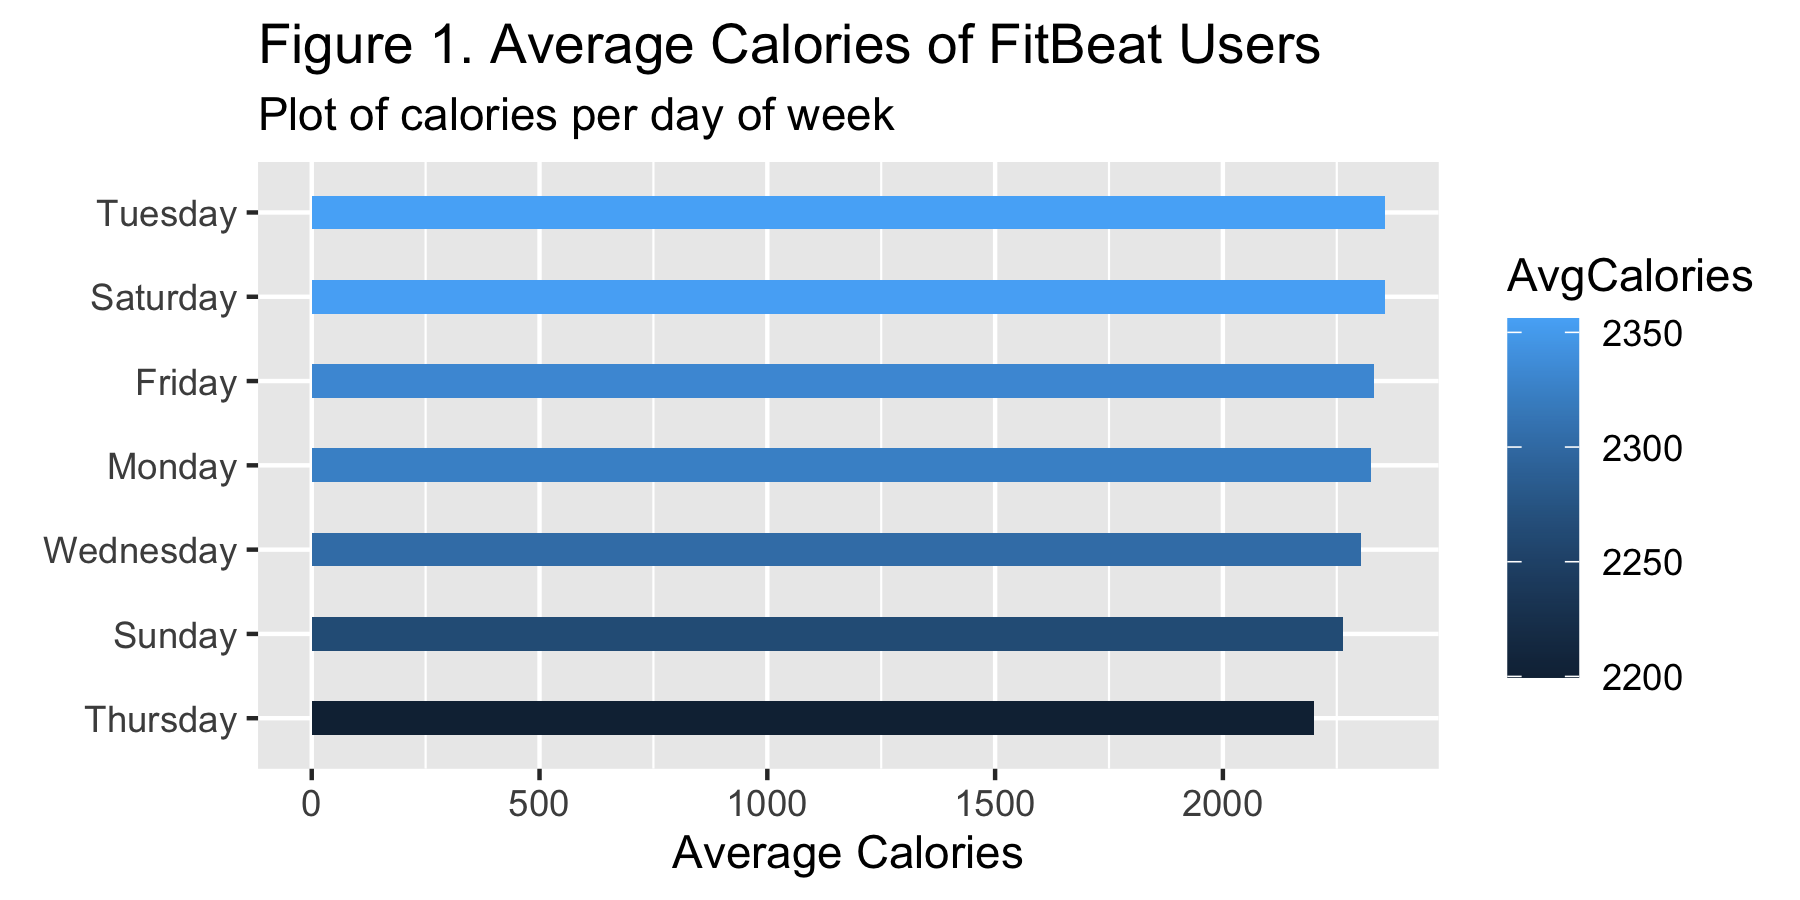
\includegraphics[width=0.9\linewidth]{./figs/barplot1} \end{center}

\begin{table}
\centering\begingroup\fontsize{14}{16}\selectfont

\begin{tabular}[t]{l}
\hline
Insights\\
\hline
The days on which users are the most active are Saturday and Tuesday.\\
\hline
Thursday and Sunday are the most passive days for users.\\
\hline
\end{tabular}
\endgroup{}
\end{table}

Note that there is no specific order in how the calories descend from
Saturday to Thursday. However, it is no surprise that Saturday users
burn the most calories and Sunday most likely take some rest. The fact
that Tuesday and Saturday are among the most active days also isn't
surprising. The bottom line is that this distribution of calories burnt
looks right intuitively.

Now, we will create a visualization that shows how the activities are
distributed per hour of each day. Figure 2 display not only the average
calories per hour, but also steps and heart rate. This will help us to
compare those three variables and see if there is an interesting pattern
at certain hours.

The range of values for calories, heart rate and steps are quite
different. Hence we will \textbf{scale/standardize} them so that they
align together. To scale these three variables I performed z-score
transformation within each variable. This means that the variables are
standardized so that the center/mean of each variable becomes 0 and the
standard deviation becomes 1, ranging all them from -3 to 3 (standard
normal). Basically the transformation removes the variation within the
variables and aligns them. Here is the formula for transformation:

\[Z_{ij} = \frac{X_{ij} -\bar{X_j}}{S_j}\]

In the formula above i and j are the indexes indicating the i-th value
of the j-th variable. \(S_j\) is the standard deviation of the \(j\)-th
variable and \(\bar{X_j}\) is the sample mean of the \(j\)th variable.

Now, we can display the resulting plot, that shows hourly calories,
steps and heart rate in hourly comparison across 7 days of week. The
dotted red line is the mean of the variables (all of them are 0). It
will help us in determining the peaks or time of the day at which the
values were away from the mean. Finally we display the plot:

\begin{center}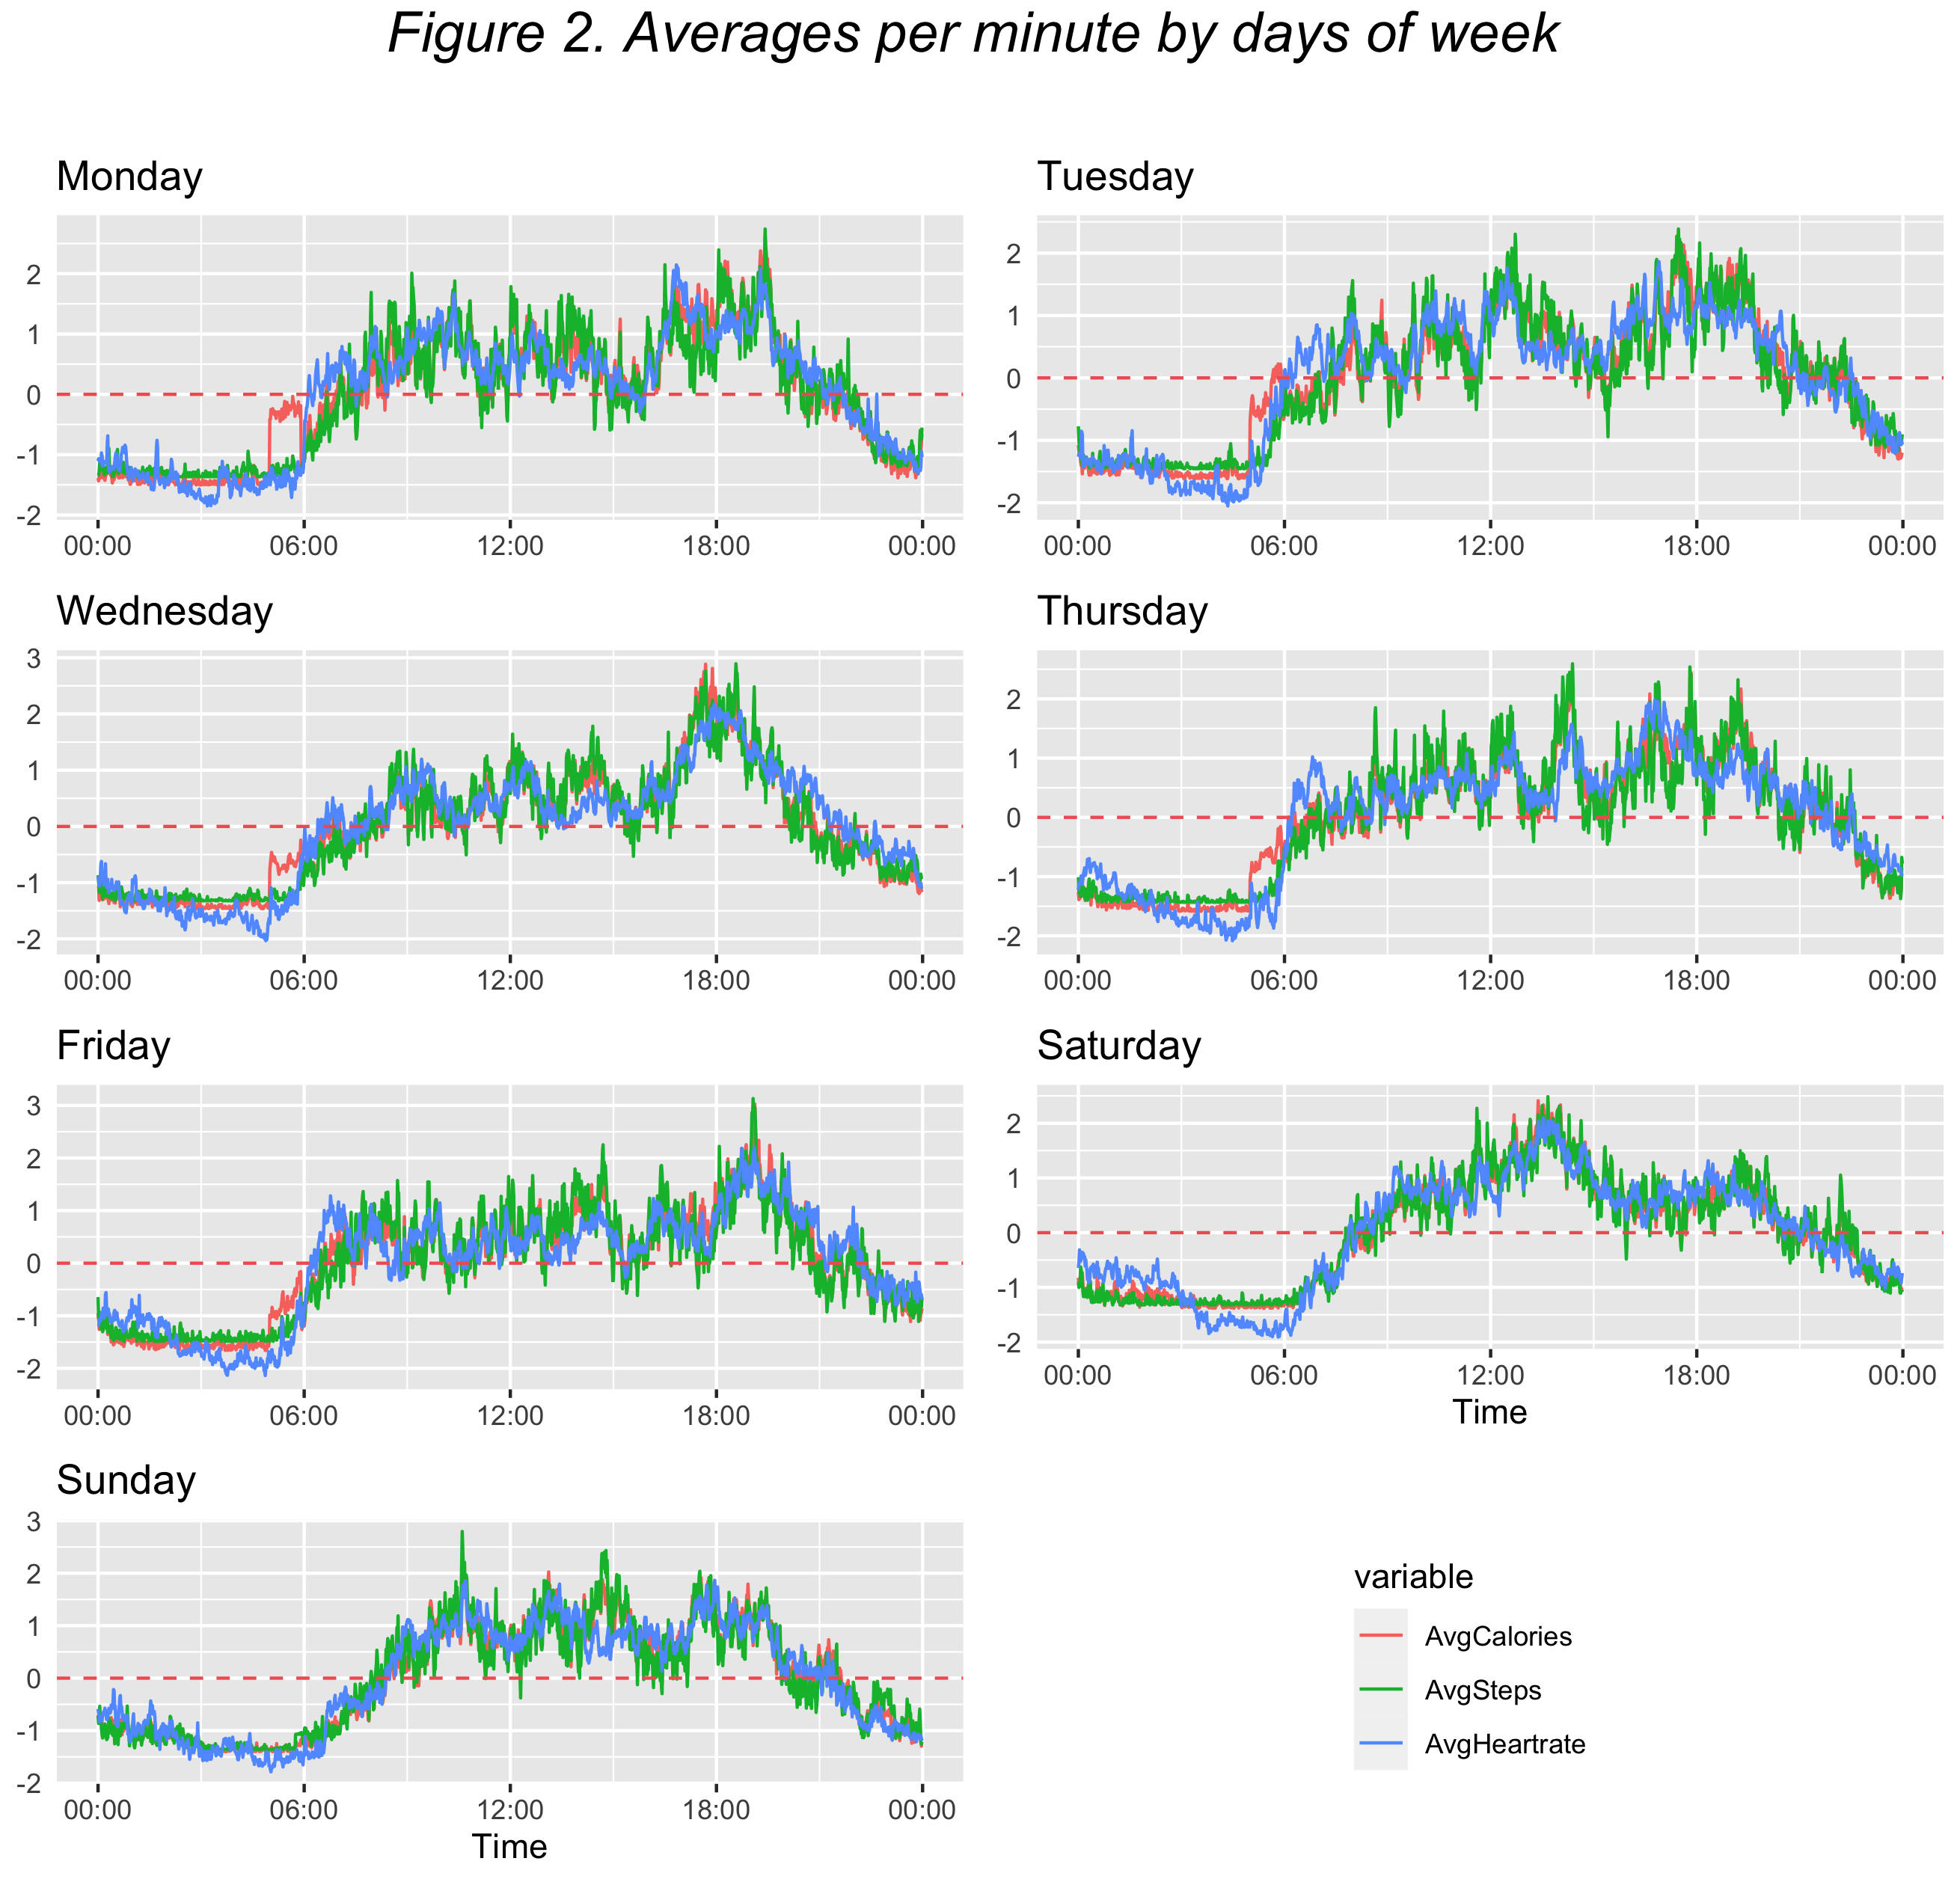
\includegraphics[width=1.1\linewidth]{./figs/lineplots1} \end{center}

\begin{table}
\centering\begingroup\fontsize{14}{16}\selectfont

\begin{tabular}[t]{l|l}
\hline
Insights & Interpretation\\
\hline
1 & From Monday to Friday,  between 5:00 and 6:00, average calories burnt run over heartrate and steps.\\
\hline
2 & From Monday to Friday,  between 6:00 and 6:30, average heartrate is relatively higher then other variables.\\
\hline
3 & The peak hours of activities mostly lie between 5:00 and 8:00.\\
\hline
4 & The peak hour for Saturday is 1:30pm.\\
\hline
5 & Tuesday doesn't have a strong peak, but rather more spread.\\
\hline
\end{tabular}
\endgroup{}
\end{table}

Insight 1 ane 2 are significant in that they show us that analyzing
these 3 variables may help us predict the type of exercise the user is
performing at a given hour. Since we know there is something interesting
happening in the morning, we will zoom in to the morning hours in the
next plot and discuss further.

Insights 3 and 4 are about the peak hours. They indicate that users are
usually performing high intensity activities in the evening. Also
Saturday the peak activities occur in the afternoon most likely because
most users do not work on Saturday.

Insight 5 tells us that, even though we determined from Figure 1 that
users are more active on Tuesday than Wednesday, Wednesday has a
stronger peak. But this doesn't mean there is a contradiction, but
rather it means that the activities on Tuesday are spread throughout the
day: In the same way that Wednesday has a stronger peak than Friday, but
the intense activities start early on Friday making it a more active
day.

Figure 2 helped us to get a clue on how the activities are distributed,
however we noticed that there is an interesting pattern eon weekday
mornings. Hence we will now zoom in to the morning part of the plot and
then compare the line-plots.

\begin{center}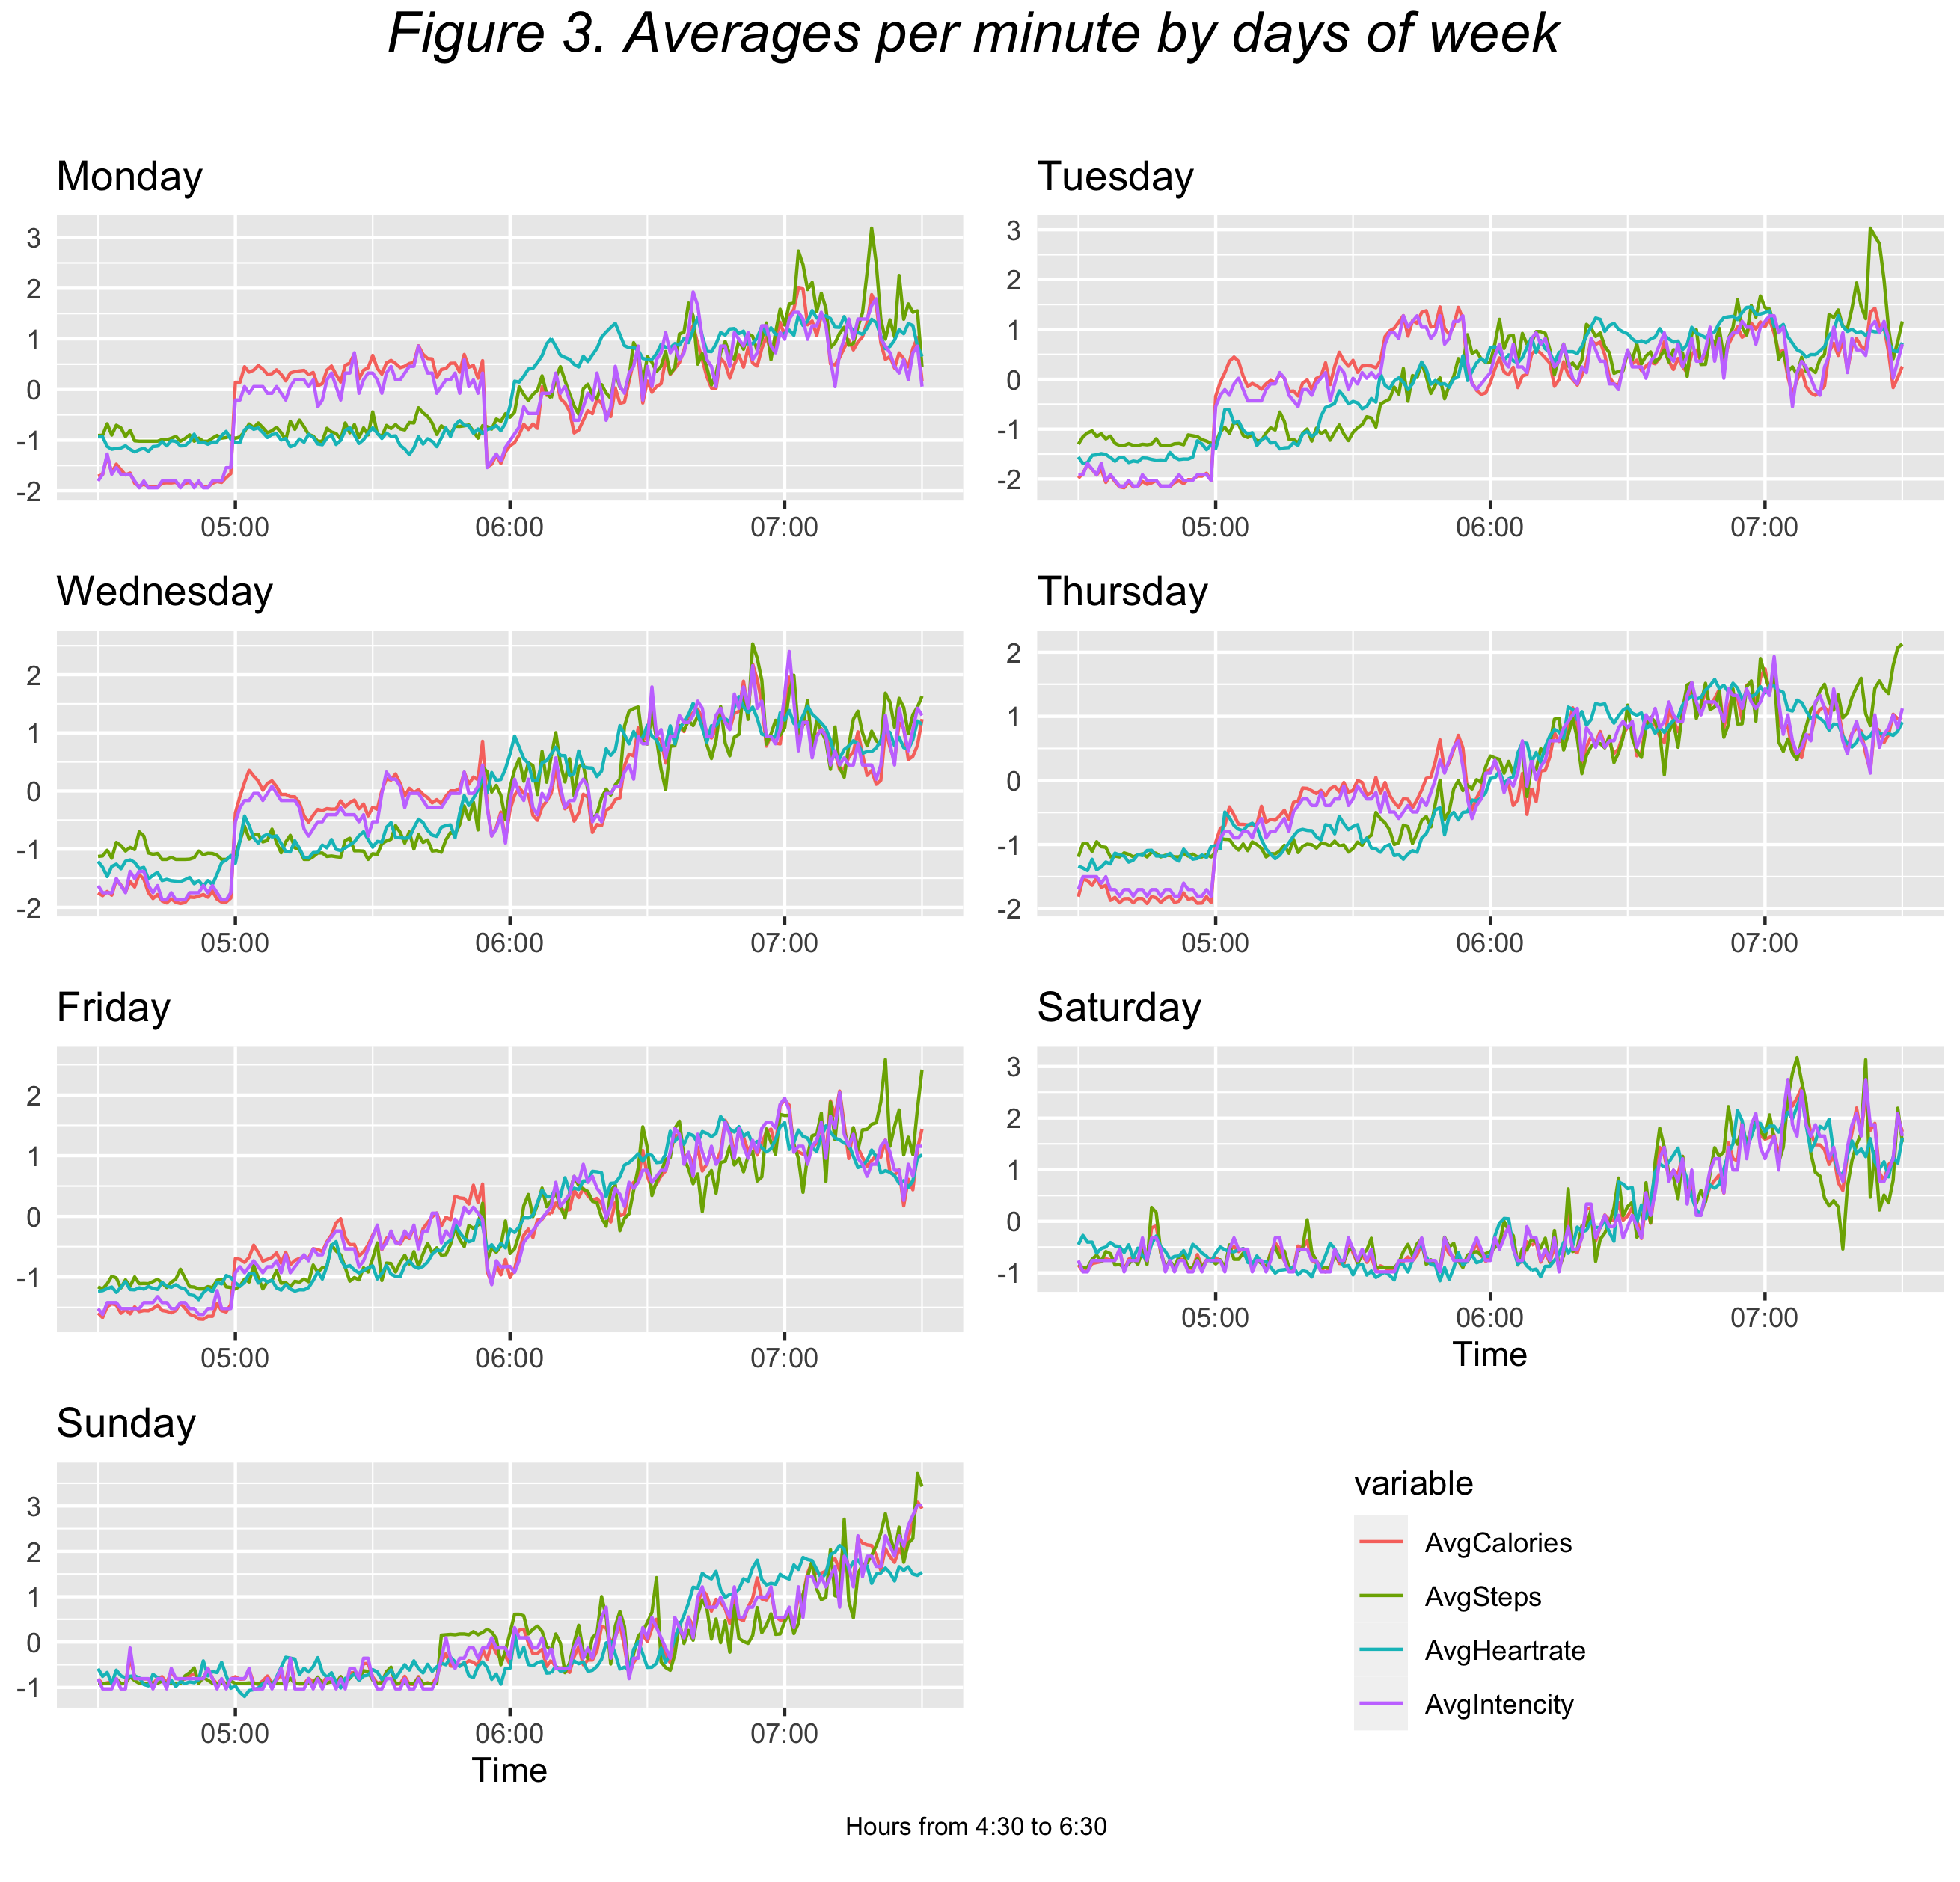
\includegraphics[width=1.1\linewidth]{./figs/lineplots2} \end{center}

\begin{table}
\centering\begingroup\fontsize{14}{16}\selectfont

\begin{tabular}[t]{l|l}
\hline
Insight & interpretation\\
\hline
1 & On weekdays between 5:00 and 6:00, average calories burnt run over heartrate and steps.\\
\hline
2 & On weekdays average calories and intencity line up well, while heartrate and steps stay low.\\
\hline
3 & On weekdays heartrate starts increasing until about 6:30\\
\hline
4 & On weekends, all the measurments line up.\\
\hline
\end{tabular}
\endgroup{}
\end{table}

It is easy to see that there is something interesting happening between
5:00 and 6:00 on the weekdays. Note that I added average intencity per
minute which is in purple color-code. Clearly, on weekday mornings
calories burnt and the intensity level have spikes and they align
together. Meanwhile, steps and heart rate stay increase gradually. There
is a contradiction here. If, for instance, users work out between 5:00
and 6:00, then at least the hart rate needs to go up with calories and
intensity. However, we know that low hart rate training such as aerobic
fitness is common in the morning. So, we may assume that users perform
morning aerobic fitness activities in the morning after which their
heart rate starts increasing as they become more energetic and ``the day
starts''. Remember that after all this plot is zoomed in and the
calories and intensity values are not that high, relative to evening
hours, for example. Of course course, when we assume that users perform
aerobic exercises, the credibility of the assumption is not perfect,
since there might be something else going on. So BellaBeat will need
collect more reliable data and involve a team of data experts to perform
controlled experiments and verify this claim by hypothesis testing.

But there is a better solution. To be fair, there is no enough
information to make conclusions on the exact type of activity users are
performing at a given hour. Although, we saw that activities performed
at each hour are associated with certain values relative to one another.
For instance, when users perform heavy weight training, intuitively,
their heart rate should be relatively higher than calories and steps. Or
when they walk, there steps should go up and heart rate stay relatively
low, and so on. So, each type of activity will generate different data
values. This means that BellaBeat can hire Data Scientists to construct
models such as \textbf{Deep Neural Network} (DNN) that learns these
associations and predicts the type of activity in real-time. To train
the DNN BellaBeat will have to collect data from users of different
qualities in such a way that the type of activity is the label for the
data generated. Then after training and completing the construction of
the DNN, BellaBeat will end up with a supervised learning model that
inputs the data recorded and outputs the type of activity the user is
performing in real time. By implementing this solution, BellaBeat will
know what activity a given user was performing, record this and give the
users alerts when they are not on the right track, or give helpful
recommendations. As a result this solution can provide users with more
valuable insights, making them trust and be more engaged with BellaBeat
app and products.

\hypertarget{correlations}{%
\paragraph{Correlations}\label{correlations}}

We already found patterns in the dataset that helped us determine some
of the daily habits of the users. Now we will analyze the relationship
between some of the other variables present in the dataset. Here I will
use some tools from traditional methods such as regression analysis.

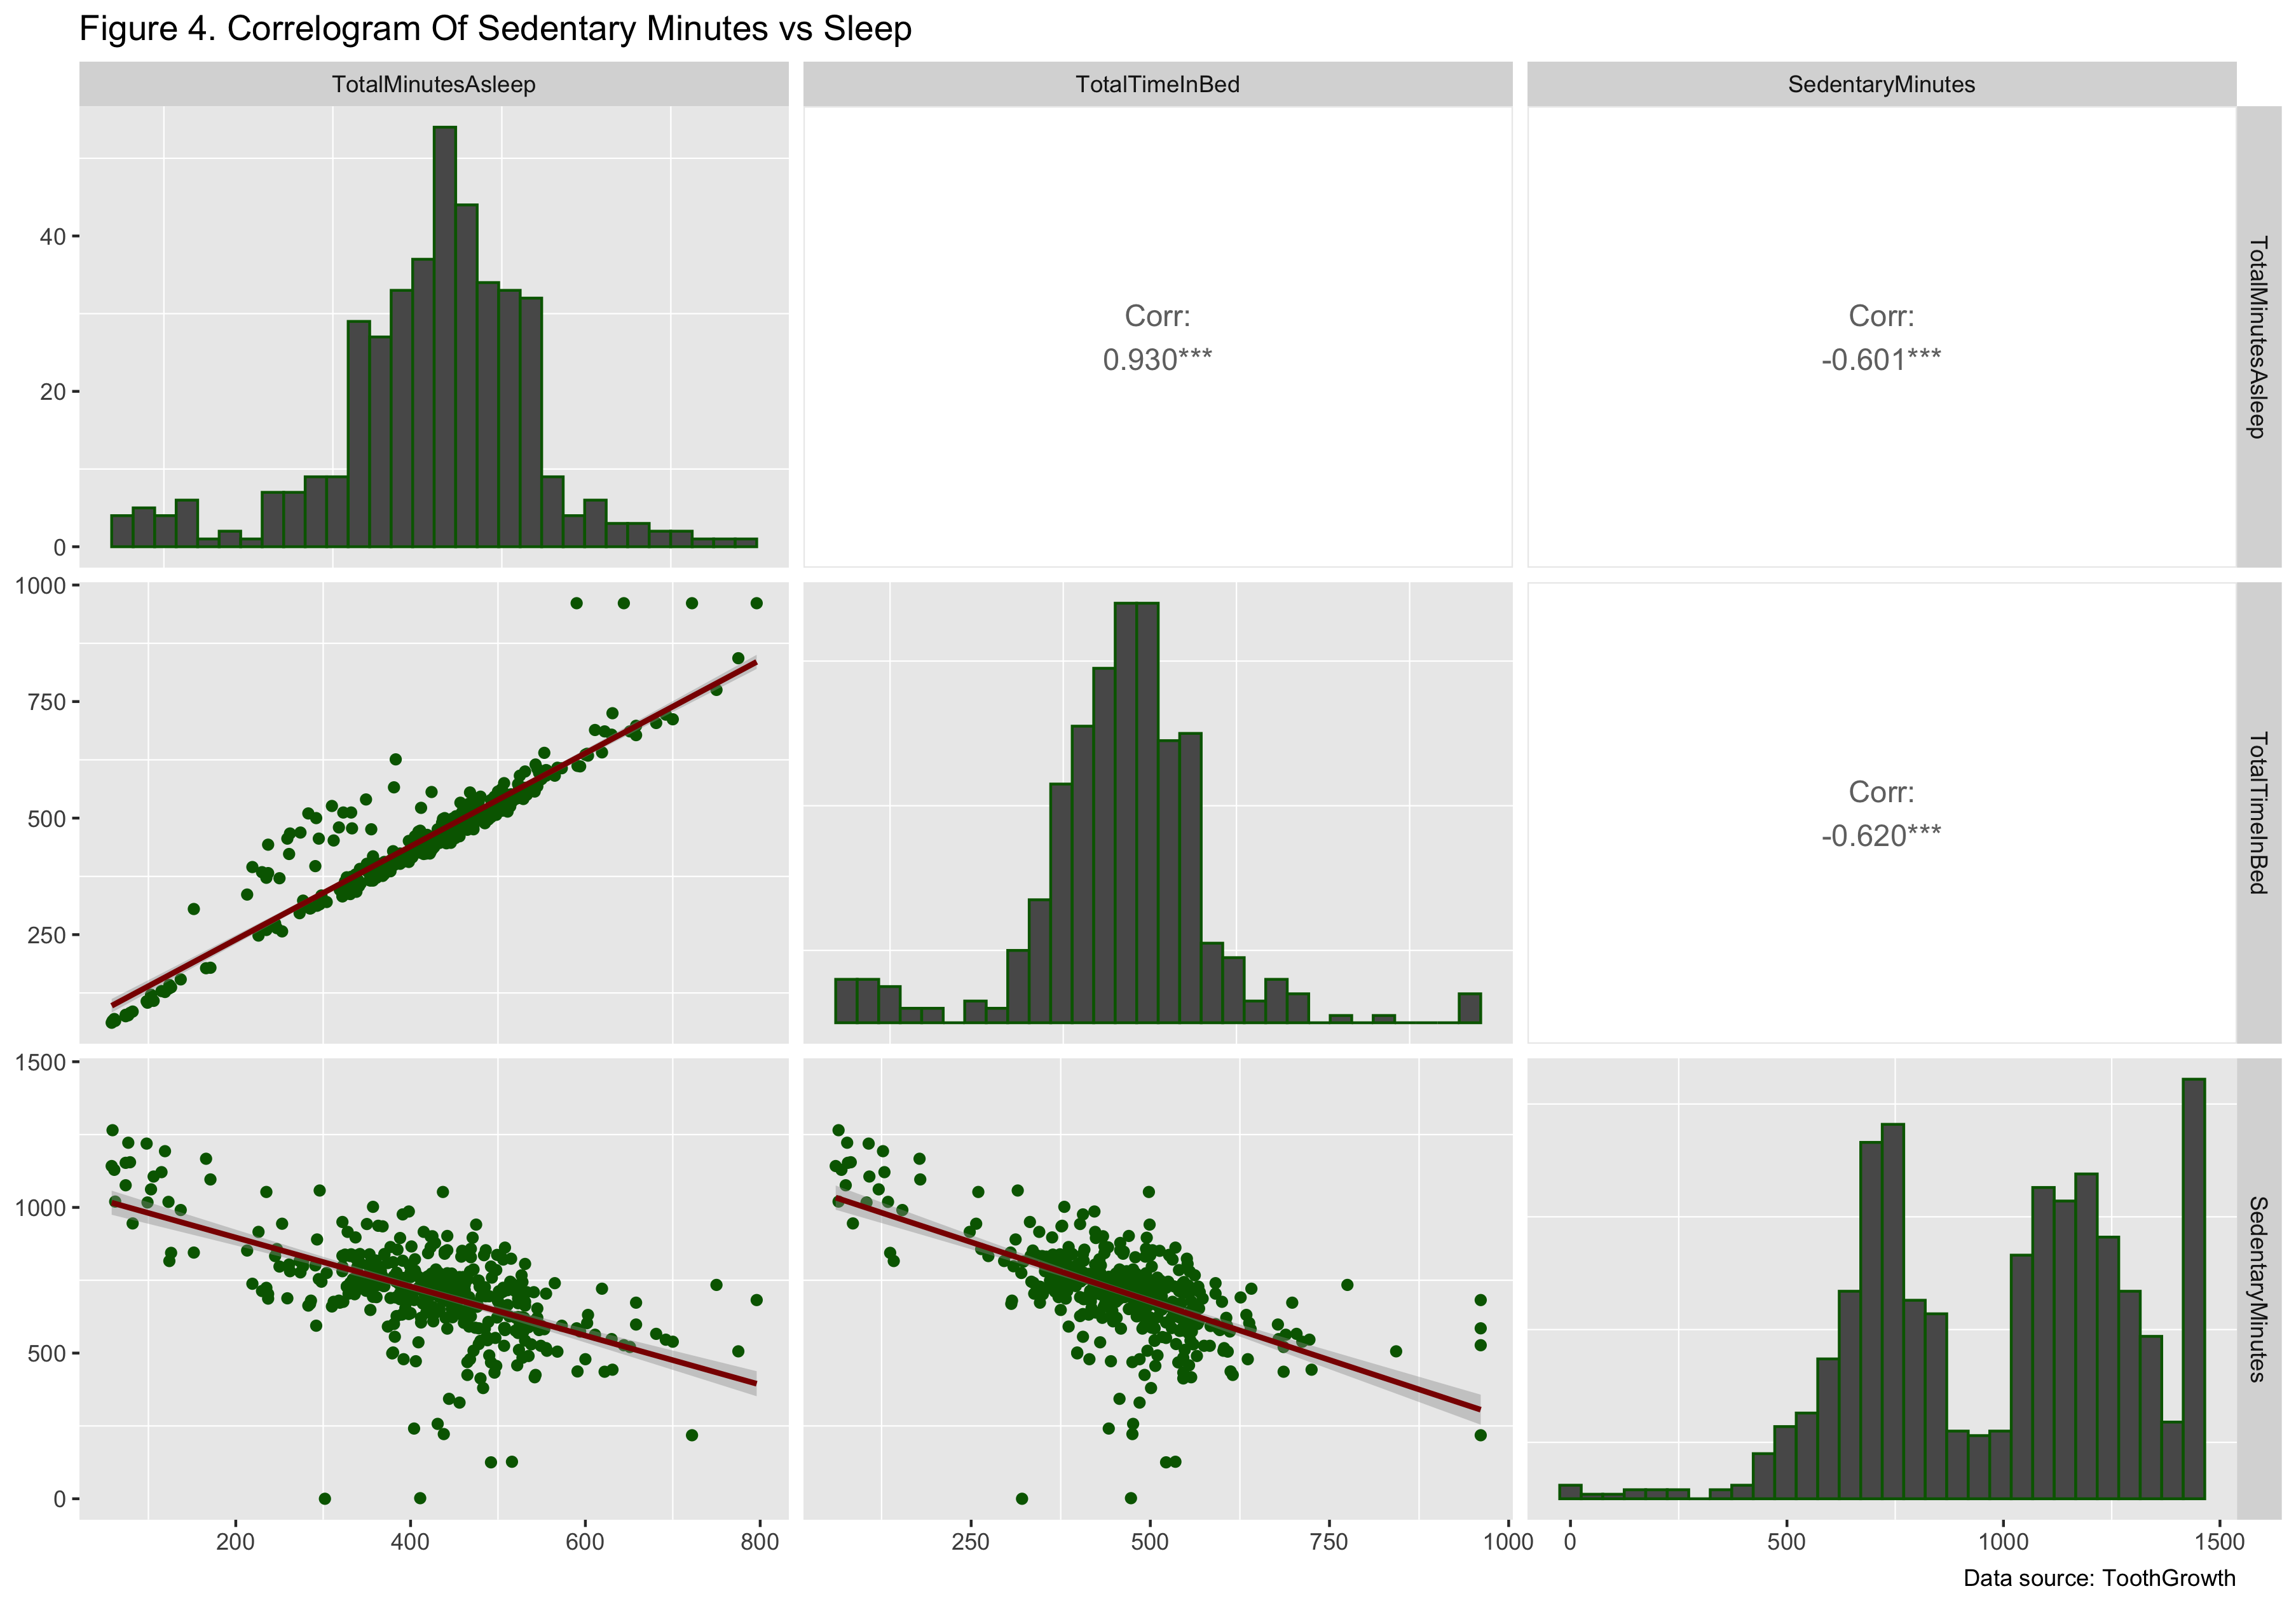
\includegraphics[width=0.9\linewidth]{./figs/correlogram1}

\begin{table}
\centering\begingroup\fontsize{14}{16}\selectfont

\begin{tabular}[t]{l|l}
\hline
Insight & interpretation\\
\hline
1 & There is a strong positive relationship between between minutes asleep and time in bed.\\
\hline
2 & Both minutes asleep and time in bed are negatively correlated with sedentary minutes.\\
\hline
3 & The distributions of minutes asleep and time in bed are approximately normally distributed.\\
\hline
4 & The distributions of sedentary minutes is bimodal.\\
\hline
\end{tabular}
\endgroup{}
\end{table}

Insight 1 tells us that users usually sleep as much as they stay in bed.
However, one can observe that there are users above the least square
regression line (red line on scatter plot TotalMiutesAsleep vs
TotalTimeInBed). This tells us that some users stay in bed without
sleeping. BellaBeat can identify those users and recommend to stay in
bed less and spend time more effectively. In the next section we will
see if we can find more associations with staying in bed.

Insight 2 is not a surprise, since it is assumed that the more people
sleep, the less they will want to spend sedentary minutes.

Insight 3, simply, suggests that most users sleep the recommended 8
hours.

Insight 4 indicates that there might be two different groups: one
spending about 700 and the other about 1200 sedentary minutes. We will
try to extract more information about those groups in the next section.

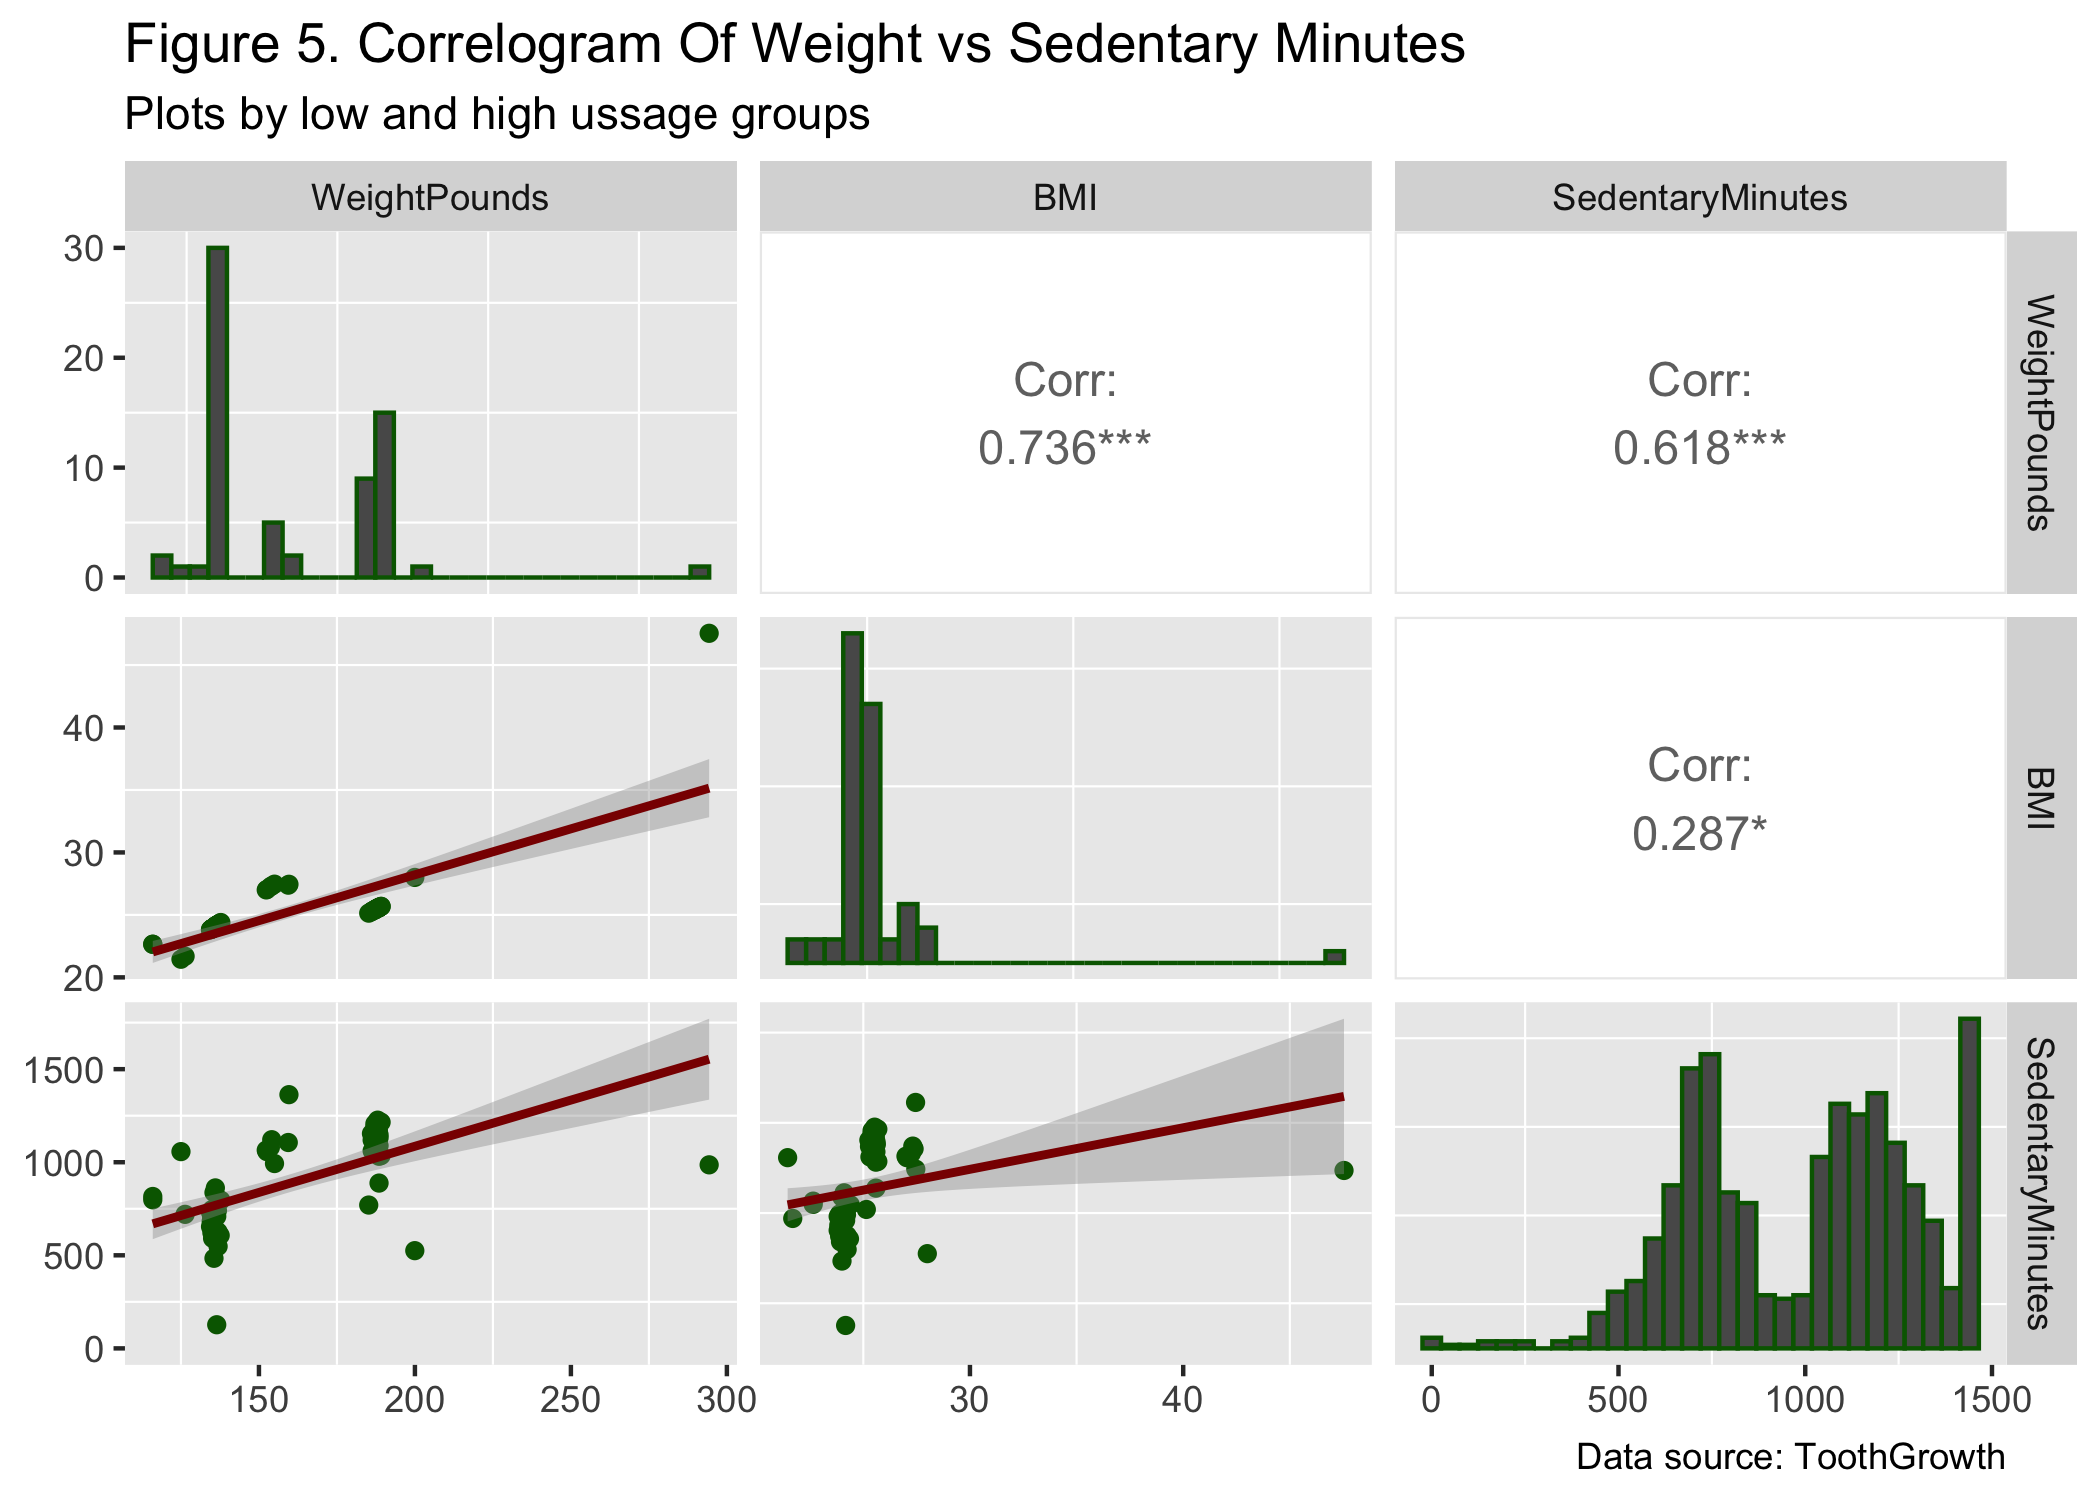
\includegraphics[width=0.9\linewidth]{./figs/correlogram2}

\begin{table}
\centering\begingroup\fontsize{14}{16}\selectfont

\begin{tabular}[t]{l|l}
\hline
Insight & interpretation\\
\hline
1 & On weekdays, between 5:00 and 6:00, average calories burnt run over heart rate and steps.\\
\hline
2 & On weekdays, average calories and intensity line up well, while heart rate and steps stay low.\\
\hline
3 & On weekends, all the measurements line up.\\
\hline
\end{tabular}
\endgroup{}
\end{table}

The insights above were gained despite the unreliable weight data. This
was done for learning purposes, but in a real world this would be
unacceptable. There are too few data points and we should not rely on
what the data tell us here. The figure itself is not satisfying. Observe
that in the top left bar plot the data is clustered around 2-3 values,
which means that not all the weight groups of the user population are
represented in the weight information. Anyways we do see a positive
correlation between weight and sedentary minutes, but we won't go any
deeper since conclusions might not be valid. Instead, in the
Recommendation section we will discuss how BellaBeat can possibly avoid
weight information issues.

\hypertarget{analyzing-high-and-low-usage-groups}{%
\paragraph{Analyzing high and low usage
groups}\label{analyzing-high-and-low-usage-groups}}

At this point we have some understanding of the data and relationships
between variables. In the process of building a machiene learning model,
data scientists will most likely group the data in different ways as
part of its feature engineering procedure. As an ilustration I picked
minutes engaged with the app as a variable to be groupped. This will
help us determine if there is a difference between people who use app
more often and those who use less.


\includegraphics[width=0.5\linewidth]{./figs/histogram1}

Observed that users' minutes spent engaging with the app is neiter
uniform or normal. Since there is no documentation on the data
collection process, we won't know the meanes or weather it was done to
adjust to the population distribution on minutes spent on the app.
Whatever it may be, it is clear that many users spent more time engaging
with the app than the rest. Hence, it is reasonable to divide users into
two categories: group of users with high usage (\textgreater40000) and
those with less (≤40000). Since calories burnt is one of the most
important variables in our dataset, we will first look at the minute
average calories burn per usage groups.

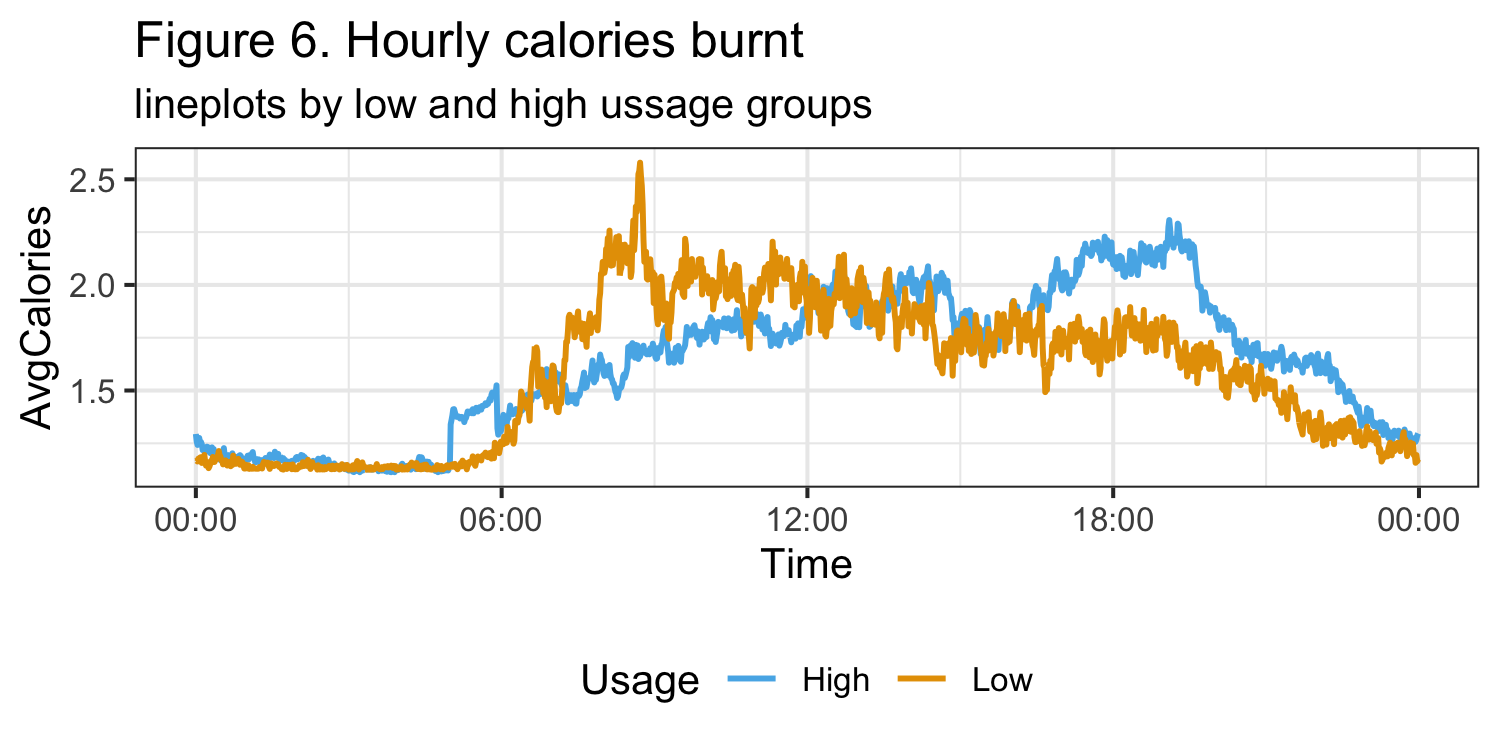
\includegraphics[width=1\linewidth]{./figs/lineplot3}

\begin{table}
\centering\begingroup\fontsize{14}{16}\selectfont

\begin{tabular}[t]{l|l}
\hline
Insight & interpretation\\
\hline
1 & The peak hour of activities for low usage groups is around 8:30.\\
\hline
2 & The peak hour of activities for high usage groups is around 18:30.\\
\hline
3 & Only High usage group has a bump in in the morning.\\
\hline
\end{tabular}
\endgroup{}
\end{table}

Insights 1 and 2 suggest that there is a clear distinction between the
two groups in terms of the time of their most intense activities during
the day. It looks like low usage group exercise in the morning, while
high usage group in the evening hours.

Insight 3 is related to the findings from Figure 1 and 2. We can observe
that only high usage group has the interesting pattern we talked about.
This means that usage may be another factor for the low heart rate
training that we discussed. We can infer that other then the 4 variables
we analyzed using Figure 2, there are other variables such as usage,
that can serve as an input the the supervised learning model we
suggested.

Now we will look at intensity levels within each group to discover other
types of variability between the groups.

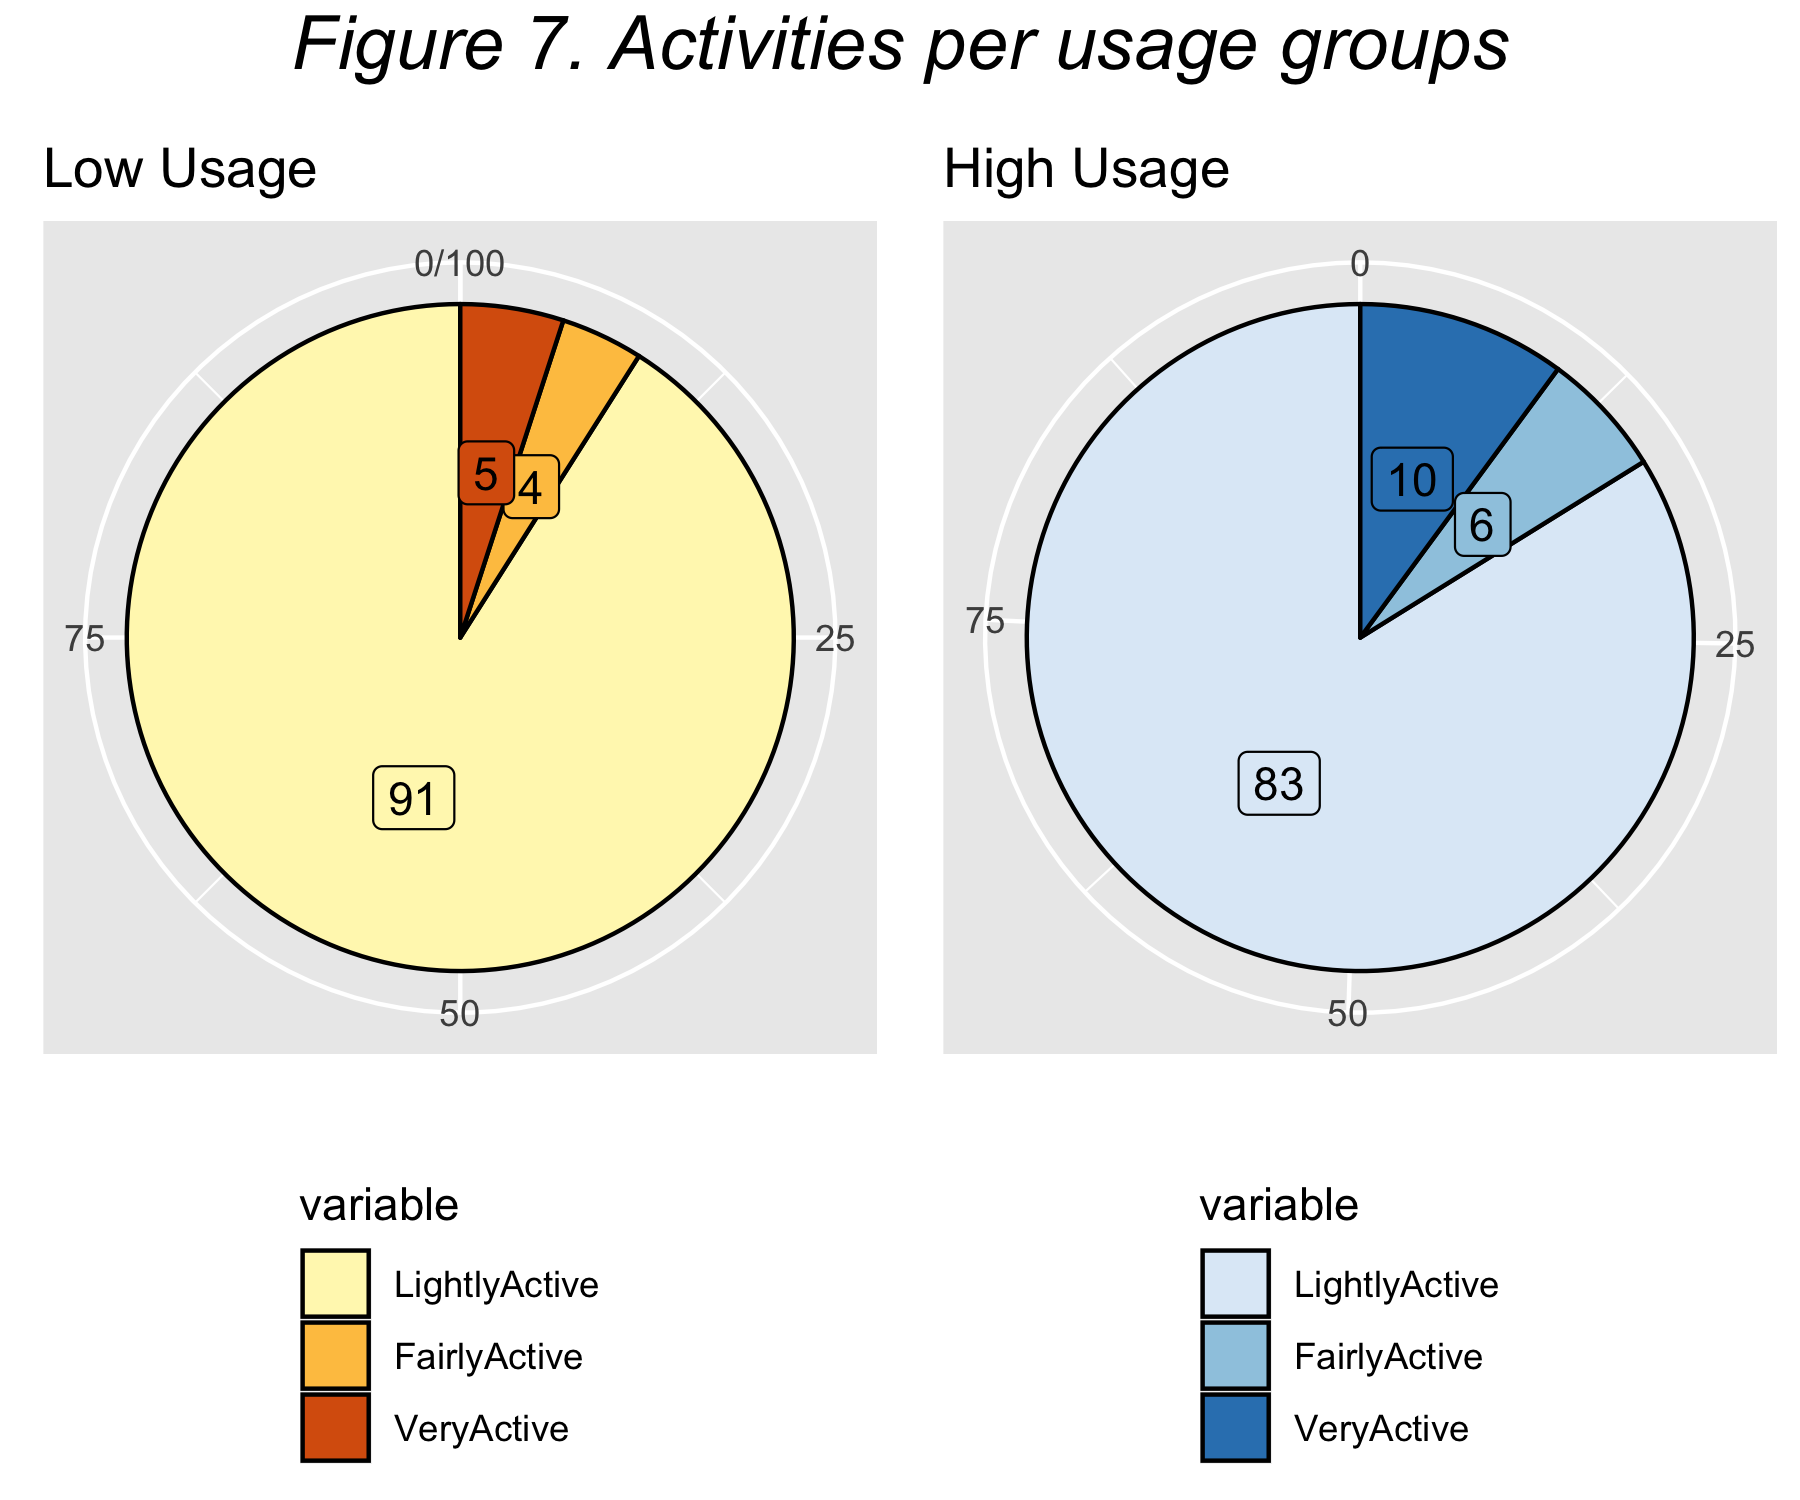
\includegraphics[width=0.6\linewidth]{./figs/pies}

\begin{table}
\centering\begingroup\fontsize{14}{16}\selectfont

\begin{tabular}[t]{l|l}
\hline
Insight & interpretation\\
\hline
1 & Low usage group users are very active 5\%, fairly active 4\% and lightly active 91\% of the times\\
\hline
2 & High usage group users are very active 10\%, fairly active 6\% and lightly active 83\% of the times\\
\hline
3 & Low usage group users are very active 5\%, fairly active 4\% and lightly active 91\% of the times\\
\hline
4 & High usage group users are very active 10\%, fairly active 6\% and lightly active 83\% of the times\\
\hline
5 & Low usage group users are very active 5\%, fairly active 4\% and lightly active 91\% of the times\\
\hline
6 & High usage group users are very active 10\%, fairly active 6\% and lightly active 83\% of the times\\
\hline
\end{tabular}
\endgroup{}
\end{table}

Those insights from the pie charts simply suggest that high usage group
is more active and spend less time in light activities. This is another
performance indicator and it indicates that the users who engage with
the app more perform better. So, the recommendation system of BellaBeat
should encourage users to be more engaged with the app.

Now, as we are analyzing the usage groups, let's inspect some
correlations per group.

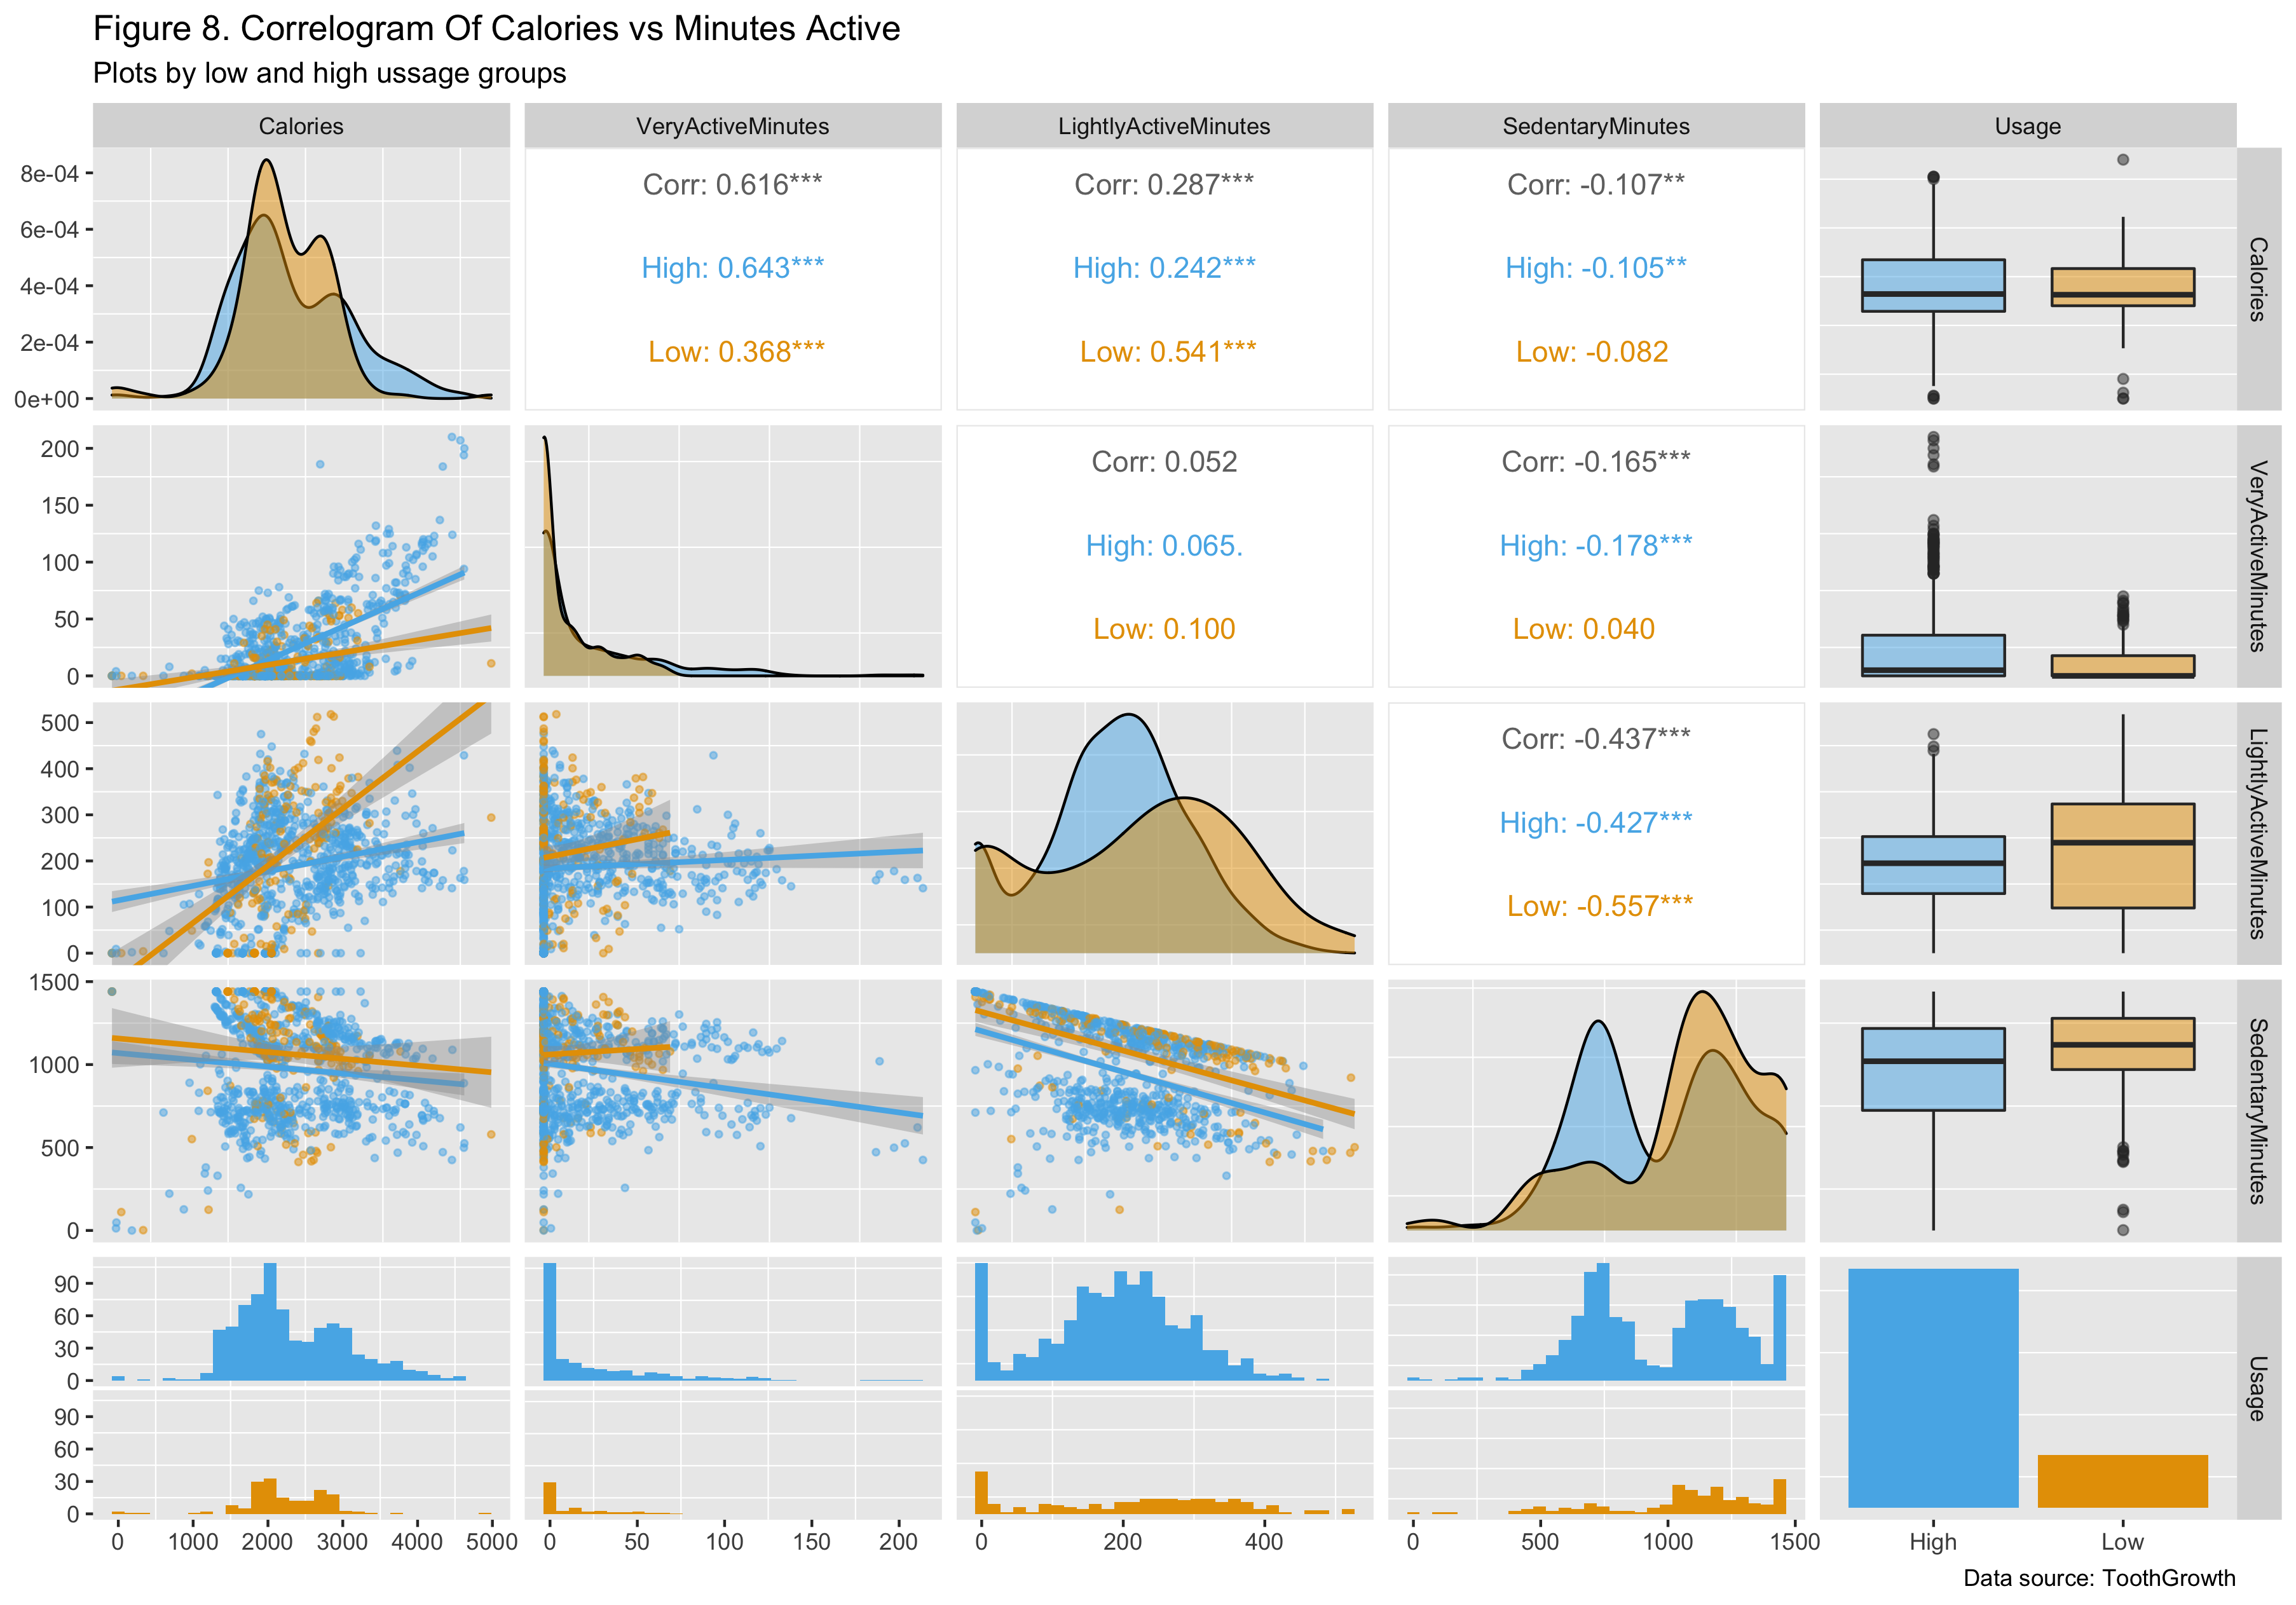
\includegraphics[width=0.9\linewidth]{./figs/correlogram3}

\begin{table}
\centering\begingroup\fontsize{14}{16}\selectfont

\begin{tabular}[t]{l|l}
\hline
Insight & interpretation\\
\hline
1 & Burning more calories by spending more very active minutes is associated with the high usage groups.\\
\hline
2 & Burning more calories by spending more light active minutes is associated with the low usage groups.\\
\hline
3 & Both light and very active minutes are correlated with calories burnt.\\
\hline
4 & Light activities are are negatively correlated with sedentary minutes.\\
\hline
5 & There are more users in high usage group than in low.\\
\hline
6 & Low usage group spends more sedentary minutes.\\
\hline
\end{tabular}
\endgroup{}
\end{table}

Insights 1, 2 are 3 are much expected and again they illustrate that the
users who engage with FitBeat products more often have higher
performance in health activities.

Insight 4 makes sense, since it claims that the more users stay lightly
active (such as walking slow) the less sedentary minutes they spend. It
also makes sense that very active minutes are not strongly correlated
with sedentary minutes, since very active minutes usually last shorter.

Because there was no documentation on the data collection procedure,
Insight 5 is not so valuable. This is because we don't know whether the
users were part of an experiment, weather they were rewarded for their
inputs or they actually represent the population of health tracker
users.

Insight 6 is also sedentary minutes but and gives rather important
information. The high usage group which is in blue produces bimodal
distribution for sedentary minutes. Whereas low usage group is more left
skewed than bimodal. This means that low usage group spends more
sedentary minutes which is not desired for healthy lifestyle. Hence this
is another reason why BellaBeat should encourage to use its products
more often.

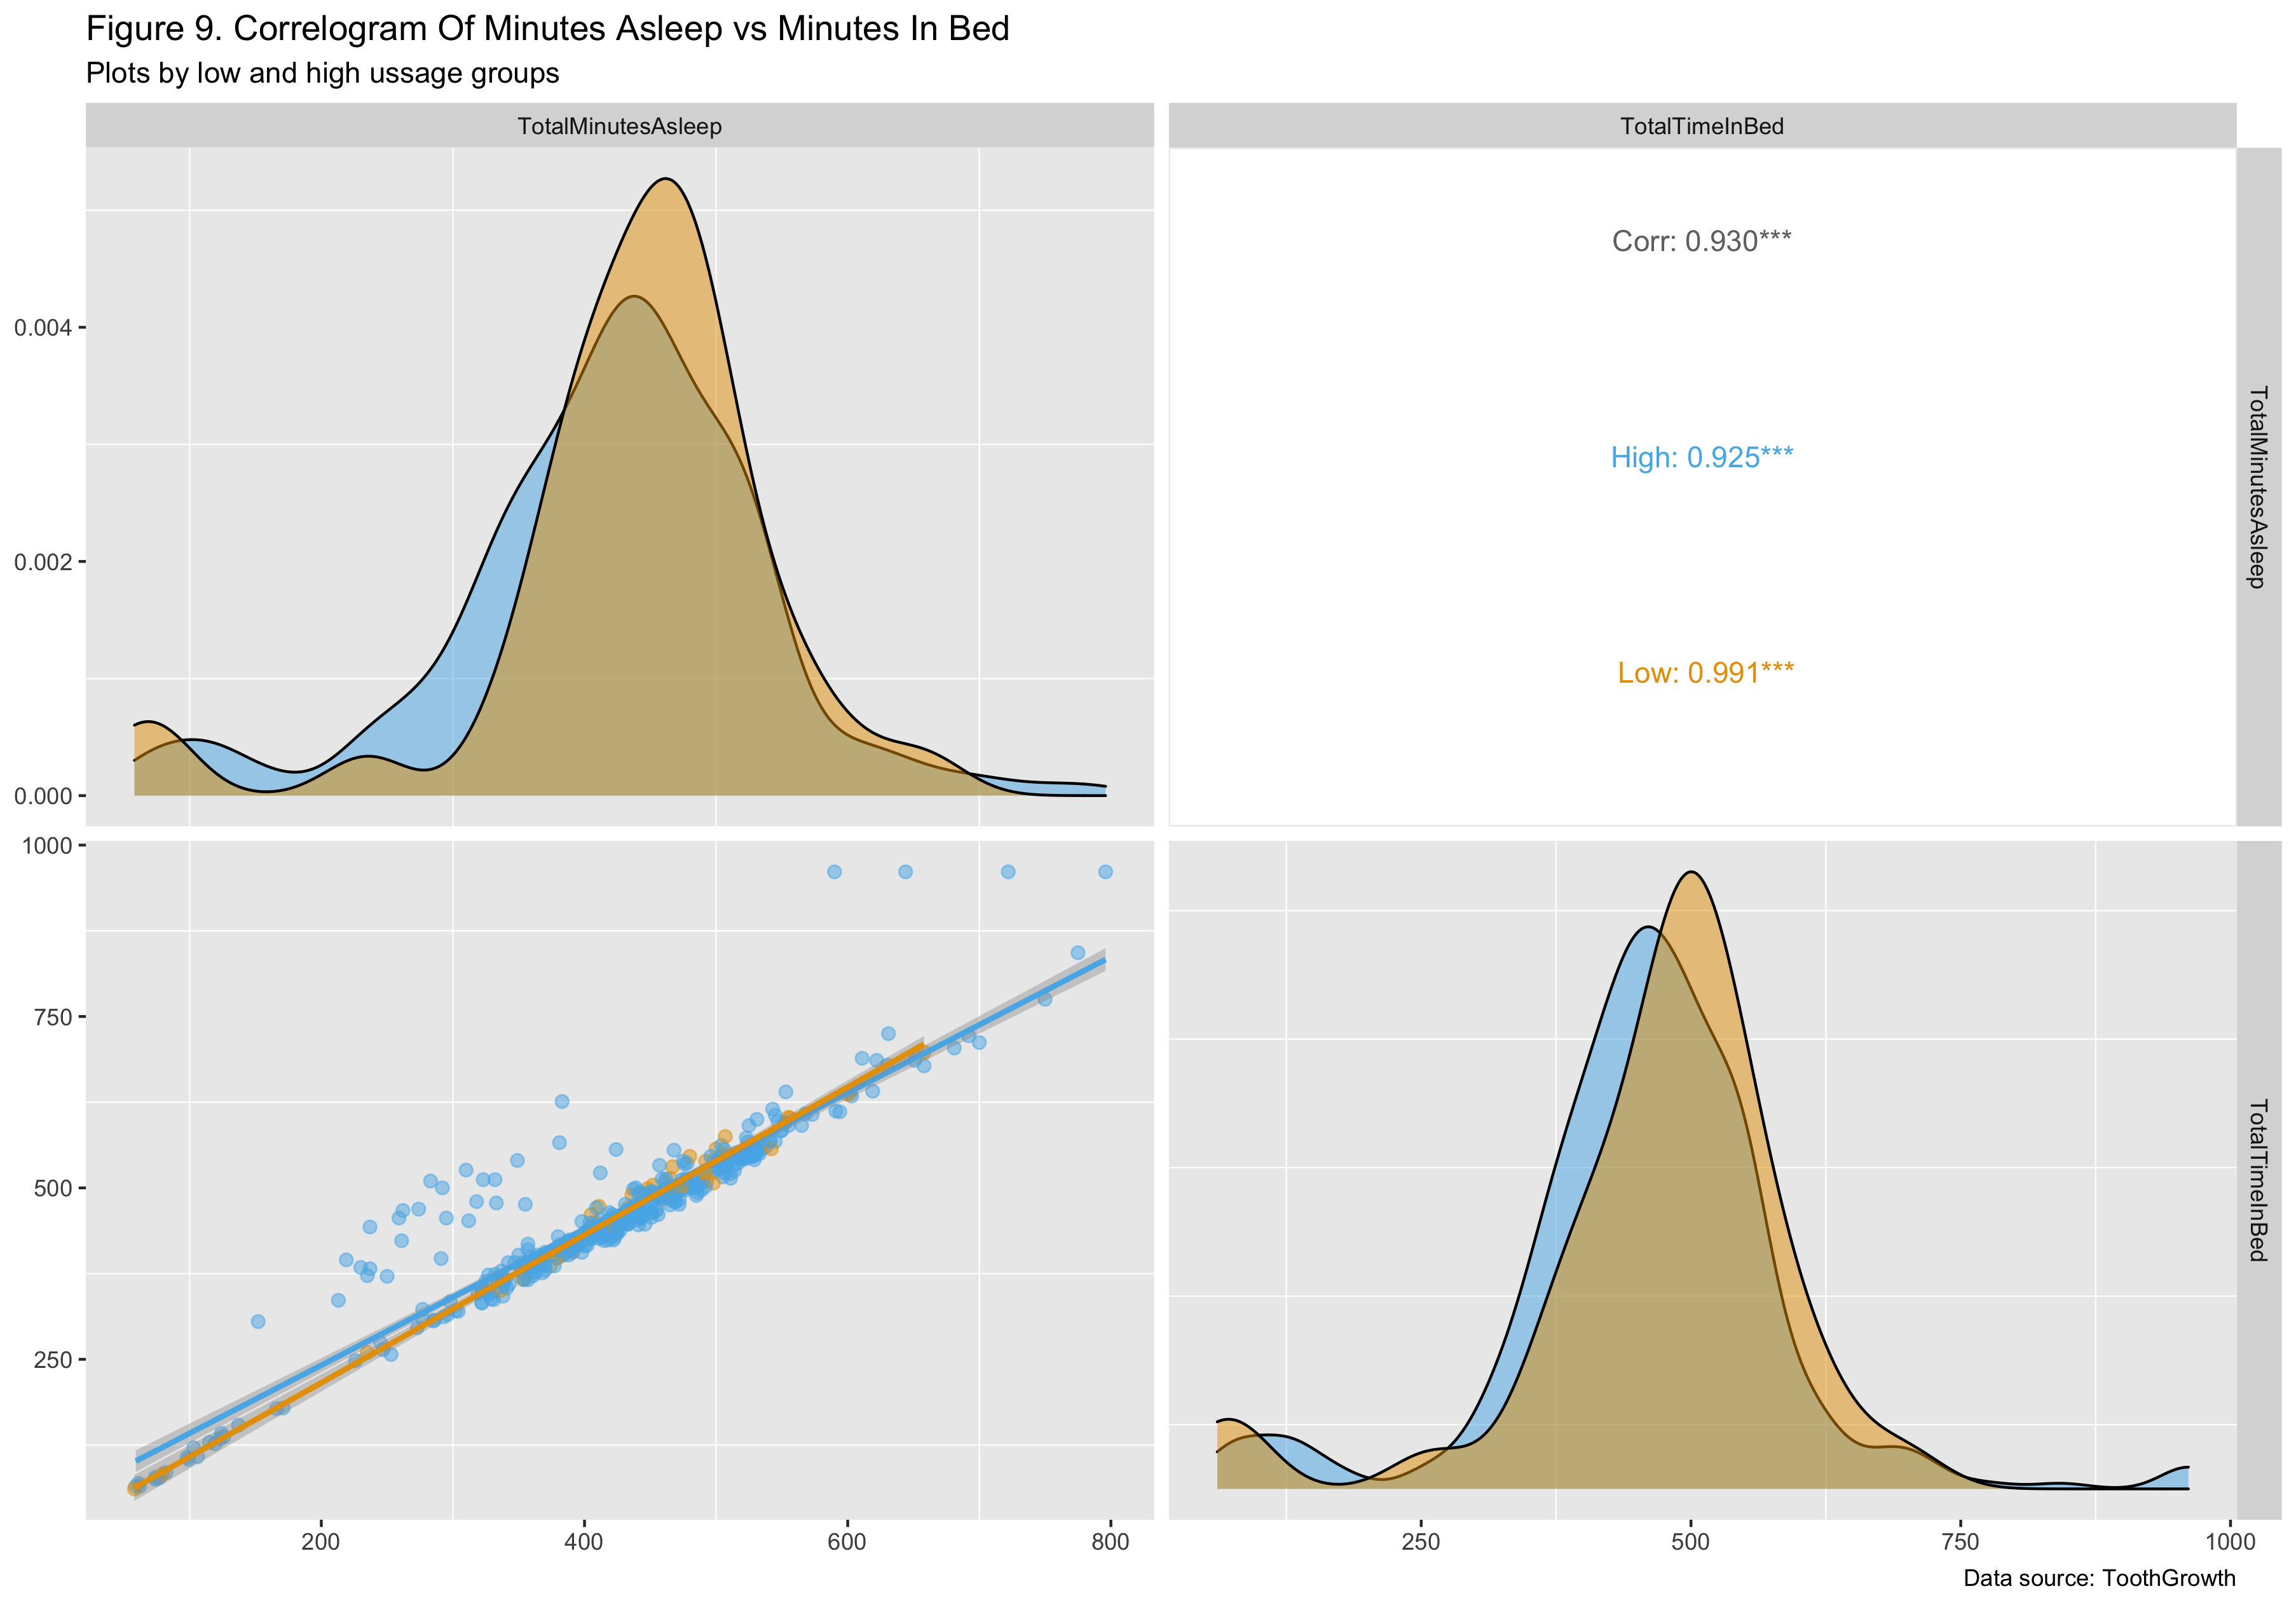
\includegraphics[width=0.9\linewidth]{./figs/correlogram4}

\begin{table}
\centering\begingroup\fontsize{14}{16}\selectfont

\begin{tabular}[t]{l|l}
\hline
Insight & interpretation\\
\hline
1 & The distribution of total minutes asleep is nearly the same for high and low usage groups.\\
\hline
2 & The distribution of total time in bed is nearly the same for high and low usage groups.\\
\hline
3 & Total time in bed and total minutes asleep are nearly collinear.\\
\hline
4 & Outliers are present only among the high usage group.\\
\hline
\end{tabular}
\endgroup{}
\end{table}

Insights 1 and 2 from figure 5 tells us that both high and low usage
group has the same sleeping patterns.

Insight 3 is clear since the lining up of the time in bed and time
asleep indicates that users usually sleep as much as they are in bed.
However, insight 4 is an indication that some users

Insight 4 tells us that the users who stay in bed more then they sleep
are among the high usage group.

\hypertarget{discussion}{%
\section{Discussion}\label{discussion}}

In this section I will discuss the most important findings and
suggestions by this case study. While working on this case study I
realized that I could build much stronger analysis and extract more
information. However, since the data integrity was violated, it was not
worth doing that. With only 33 users and 30-day user data, we wouldn't
be able to get the big picture and produce accurate results. There are
important variables such as weather within each season or variability of
user characteristics, which can not be ignored. After all, the fact that
the data is bad makes results of any analysis unreliable. However, even
with the limited data we were able to see how relationships betweem
variables can be a proper ground for building machiene learning models.
We were also able to determine data issues and ways to avoid them.
Hence, this analysis can be valuable for the marketing team at
BellaBeat, in that they can use it to prioritize their marketing
campaigns. That is the marketing team needs to focus on resolving the
most important issues related to data.

Perhaps, one of the most important suggestion here is that, as mentioned
before, Bellabeat should focus on integrating data science into its
recommendation system. We need to refer to a market research, but it can
be assumed that what users want is probably an app that helps them track
their progress accurately and help them reach their goals effectively.
Data scientists can develop classification algorithms such as neural
network that will accurately predict the type of activity at a given
time. Of course, the recommendation system will have more components
then a single classification model. It should have multiple models and
connections so that the system is robust and provides with many more
valuable insights than simply predicting the type of activity. For
example, BellaBeat can use this predictions to make suggestions on how
its users can perform the predicted type of activity effectively
(weather it is a workout or an evening walk). To do so, BellaBeat needs
to gather a team of experts, including data engineers, data scientists,
researchers and more. The bottom line is that the results from this case
study suggest that from data perspective there is a ground for
implementing such solutions. This is because, analyzing FitBeat data, we
saw that the activity patterns clearly vary across different hours of
the day. In addition, to implement these data science solutions
BellaBeat will need to gather reliable training and testing and
validation datasets. A ballpark figure is that experiments should be
conducted where participants do different activities and collect data
along with the label identifying the type of activity.

Another suggestion, that should not be ignored, refers to the data
engineering process. We saw that the data issues that violated the its
integrity resulted in lots of problems throughout this case study.
Robust recommendation system such as the one we discussed will not work
if the data is not reliable. Hence, data engineers must make sure that
the integrity is not violated. First of all, they must provide with a
sufficient documentation of the data engineering process. This will help
data analysts and data scientists to trace back and find answers in case
there is a need to. It is understandable that gathering user information
such as weight can be challenging. However, BellaBeat can develop a
solution that offers users a smart body weight scale that records their
weight periodically. Then the scale can transfer data to BellaBeat app
when the final measurement is approved by the user. Doing so will
prevent human errors and make the weight information more consistent.
Secondly, they need to make sure that all the observations are gathered
simultaneously within seconds. This will help BellaBeat avoid
inconsistencies in the observation times. There are a lot of other
issues that can violate data integrity and give users inaccurate
information. These issues must simply be resolved for a proper use of
data.

We also discovered that there were correlations between many of the
variables in the dataset. This is again an indication that there is a
potential ground for data science procedures. Correlation between
variables such as weight and sedentary minutes, or calories and the
level of intensity can be extremely valuable for the recommendation
system of BellaBeat app. The downside of case studies like this one is
that it can not be used to determine cause and effect relationships
between variables. For instance knowing that there is a relationship
between the minutes of user engagement with the app and the level of
intensity of the activities does not tell us which one is caused by the
other. Finding the cause could help us recommend users to engage in
certain activities for their health improvements. However, building
classification models can solve those problems, because then, when there
is a robust recommendation system, these causes will not matter; the
only thing that matters will be accurate recommendations that lead users
to success.

\hypertarget{recommendations}{%
\section{Recommendations}\label{recommendations}}

In the previous section we discussed how the findings from this case
study relates to BellaBeat users. We also gave thorough suggestions on
what can be done to improve BellaBeats decision making, using data, and
how they can avoid issues related to data integrity and error-free
recommendation system. In this section we will give the summary of high
level suggestions related to the most important findings in this case
study.

\begin{itemize}
\tightlist
\item
  Integrate data science into BellaBeats recommendation system.
\item
  Assign data engineers to focus on collecting the most valuable
  information, without violating data integrity.
\item
  Partner up with a smart scale company to develop a smart scale
  solution that integrates into BellaBeat app and records weight
  information accurately.
\item
  While collecting data from users include a thorough documentation on
  the collection process.
\item
  Encourage users to spend more time engaging with the app.
\end{itemize}

\hypertarget{references}{%
\section{References}\label{references}}

\textbf{The analysis and code used here can be found on Github:}

GitHub Repository:

\textbf{The data privacy information can be found:}

Fitness tracker's data privacy:
\url{https://openeffect.ca/fitness-trackers/Fitness_Tracker_Questions.pdf}

BellaBeat's privacy policy: \url{https://bellabeat.com/privacy-policy/}

\textbf{The data set can be found on Kaggle:}

Kaggle link: \url{https://www.kaggle.com/arashnic/fitbit}

\textbf{Google Data analytics:}

Case Study Guidelines:

Coursera link:
\url{https://www.coursera.org/professional-certificates/google-data-analytics}

\end{document}
